\documentclass[11pt]{article}

\usepackage[a4paper,margin=0.72in]{geometry}
\usepackage{amsmath,amssymb,mathtools}
\usepackage{graphicx}
\usepackage{subcaption}
\usepackage{booktabs}
\usepackage{array}
\usepackage{float}
\usepackage{enumitem}
\usepackage{hyperref}
\usepackage{xcolor}

\captionsetup{font=small,skip=3pt}
\captionsetup[subfigure]{font=scriptsize,skip=1pt}

\newcolumntype{L}[1]{>{\raggedright\arraybackslash}p{#1}}
\newcommand{\R}{\mathbb{R}}
\newcommand{\norm}[1]{\left\lVert #1 \right\rVert}
\newcommand{\F}{\mathrm{F}}
\newcommand{\op}{\mathrm{op}}
\newcommand{\Muon}{\mathrm{Muon}}
\newcommand{\GD}{\mathrm{GD}}
\newcommand{\one}{\mathrm{1step}}

\hypersetup{
  colorlinks=true,
  linkcolor=blue!50!black,
  citecolor=blue!50!black,
  urlcolor=blue!50!black
}

\title{One-Step Recovery in Gaussian Associative Memory:\\
Best One-Step Sweeps and Convergence-Reference Fractions}
\author{}
\date{}

\begin{document}
\maketitle

\begin{abstract}
This report studies whether a single update already learns the dominant
structure in the Gaussian associative-memory problem.  The first experiment
compares the best one-step full-batch update obtainable by sweeping a dense
learning-rate grid for gradient descent (GD) and spectral descent, which we
use as the exact aggregate polar-direction proxy for Muon.  The second
experiment asks a sharper question: for each largest feasible
$(\alpha,\beta,d)$ setting, how much of a separately optimized convergence
reference is already achieved by the best one-step update?  Across the
computationally accessible regimes, one step captures a large fraction of
the optimized loss improvement and weighted recovery.  The larger-$\beta$
blocks should be read as conservative evidence because exact all-pairs
evaluation forces the dimension $d$ to be much smaller there; with larger
$d$, the recovery picture is expected to improve in the regimes predicted by
theory.
\end{abstract}


\section{Problem setup}

\subsection{Gaussian associative memory}

For each tuple $(d,\beta,\alpha,\mathrm{seed})$, we generate
\[
  N=\mathrm{round}(d^\beta)
\]
memory pairs
\[
  u_i,v_i\sim_{\mathrm{iid}}\mathcal{N}(0,I_d/d),
  \qquad i=1,\ldots,N.
\]
The item weights follow a Zipf law
\[
  p_i=\frac{i^{-\alpha}}{\sum_{k=1}^N k^{-\alpha}},
\]
with $p_i=1/N$ at $\alpha=0$.

For a matrix $W\in\R^{d\times d}$, the exact weighted full-softmax loss is
\[
  L(W)
  =
  \sum_{i=1}^N p_i
  \log\left(
    \sum_{j=1}^N
    \exp(u_j^\top Wv_i)
  \right)
  -
  \sum_{i=1}^N p_i u_i^\top Wv_i .
\]
At initialization $W_0=0$, all logits are equal and therefore
\[
  L(W_0)=\log N.
\]

\subsection{One-step directions}

Let $G=-\nabla L(0)$ be the negative full-batch gradient at initialization.
In this model,
\[
  G=\sum_{i=1}^N p_i(u_i-\bar u)v_i^\top,
  \qquad
  \bar u=\frac1N\sum_{j=1}^Nu_j .
\]
The one-step GD direction is
\[
  D_{\GD}=\frac{G}{\norm{G}_{\F}}.
\]
Let $G=P\Sigma Q^\top$ be an SVD.  The one-step spectral direction is
\[
  D_{\Muon}=PQ^\top .
\]
This is the exact aggregate polar direction.  Throughout the report,
``Muon/Spectral'' refers to this one-step spectral descent proxy.  For each
direction $D$, Experiment~I evaluates the one-step ray
\[
  W(\eta)=\eta D
\]
over a dense positive learning-rate grid and records the best one-step
outcome.

\section{Experiment design}

\subsection{Grid}

Both experiments use 10 seeds and 16 explicitly swept alpha values:
\[
  \alpha\in
  \{0,0.1,0.25,0.35,0.5,0.65,0.75,0.9,
  1.0,1.1,1.25,1.5,1.75,2.0,2.5,3.0\}.
\]
The $d$ values vary with $\beta$ because exact all-pairs recovery evaluation
requires evaluating $N^2$ logits.  The largest exact-computable $d$ is large
for low $\beta$ and necessarily small for high $\beta$.

\begin{table}[H]
\centering
\caption{Largest exact-computable $d$ used in each $\beta$ block.  Because
exact all-pairs recovery evaluation scales with $N^2$, larger $\beta$ forces
the experiment to use much smaller $d$.}
\small
\begin{tabular}{rrr}
\toprule
$\beta$ & largest $d$ & $N$ \\
\midrule
0.50 & 512 & 23 \\
0.75 & 512 & 108 \\
1.00 & 512 & 512 \\
1.25 & 512 & 2435 \\
1.50 & 512 & 11585 \\
1.75 & 128 & 4871 \\
2.00 & 96 & 9216 \\
2.25 & 48 & 6064 \\
2.50 & 32 & 5793 \\
3.00 & 20 & 8000 \\
4.00 & 10 & 10000 \\
\bottomrule
\end{tabular}
\label{tab:grid-d-limits}
\end{table}

\subsection{Experiment I: best one-step sweep}

Experiment~I is the original one-step experiment.  For every feasible
$(d,\beta,\alpha,\mathrm{seed})$ instance and for each method
$D\in\{D_{\GD},D_{\Muon}\}$, we evaluate a dense learning-rate grid along
$\eta D$.  The loss metric is reported at the best loss learning rate.
Hard recovery metrics are rank-based and therefore depend only on the
positive ray direction.  The completed run contains 13,980 method-instance
rows, with 6,990 GD rows and 6,990 Muon/Spectral rows.

\subsection{Experiment II: convergence-reference fraction}

Experiment~II keeps the same largest-$d$ grid and changes the comparison
target.  Instead of only comparing GD and Muon/Spectral one-step updates
against each other, it compares each one-step result with a separately
optimized convergence reference for the same
$(\beta,\alpha,\mathrm{seed})$.  The reference is obtained by mini-batch
AdamW training, while all reported reference metrics are still measured by
exact all-pairs evaluation.

Thus the main quantity in Experiment~II is a fraction:
\[
  \frac{\text{best one-step performance}}
       {\text{best observed convergence-reference performance}}.
\]
This directly measures how much room remains after one step.  The final
reference table contains 1,760 rows: 11 beta values, 16 alpha values, and 10
seeds.  Fractions are not clipped, and small nonzero denominators are kept.

\subsection{Reading the large-$\beta$ blocks}

For large $\beta$, the exact experiment can only use much smaller $d$; see
Table~\ref{tab:grid-d-limits}.  Therefore the Experiment~I recovery values in
these blocks are conservative.  When low-alpha, large-$\beta$ cells look
weak, the main limitation is that the available $d$ is not large enough, not
that the experiment has discovered a genuine need for many optimization
steps.

\section{Metrics}

\subsection{One-step metrics}

For any matrix $W$, define the logits
\[
  s_{ji}(W)=u_j^\top Wv_i .
\]
For item $i$, the correct logit is $s_{ii}(W)$.  Define
\[
  \mathrm{rank}_i(W)
  =
  1+\#\{j\ne i:s_{ji}(W)\ge s_{ii}(W)\}.
\]
Item $i$ is hard recovered when $\mathrm{rank}_i(W)=1$.  For a positive
one-step ray $W=\eta D$, this event is independent of the scale $\eta$.

\paragraph{Weighted hard recovery.}
The main recovery metric is
\[
  \mathrm{WHR}(W)
  =
  \sum_{i=1}^N p_i\,\mathbf{1}\{\mathrm{rank}_i(W)=1\}.
\]
This is the primary task-relevant recovery metric because the loss weights
item $i$ by $p_i$.

\paragraph{Hard count recovery.}
The unweighted count recovery metric is
\[
  \mathrm{HCR}(W)
  =
  \frac1N\sum_{i=1}^N \mathbf{1}\{\mathrm{rank}_i(W)=1\}.
\]
This is stricter than weighted recovery: it asks whether most memories are
recovered, not only whether most probability mass is recovered.

\paragraph{Weighted soft recovery.}
Let
\[
  q_i(W)=
  \frac{\exp(s_{ii}(W))}
  {\sum_{j=1}^N\exp(s_{ji}(W))}
\]
be the full-softmax probability assigned to the correct memory for query
$v_i$.  The weighted soft recovery metric is
\[
  \mathrm{WSR}(W)=\sum_{i=1}^N p_i q_i(W).
\]
Unlike hard recovery, this metric depends on the scale of $W$.

\paragraph{Loss-drop fraction.}
For a one-step method, let $\eta_{\rm loss}$ be the best learning rate in
the sweep for minimizing $L(\eta D)$.  The one-step loss-drop fraction is
\[
  \mathrm{LDF}_{\one}
  =
  \frac{\log N-L(\eta_{\rm loss}D)}{\log N}.
\]
A value near 1 means that one step removes nearly all of the initial
cross-entropy loss.

\subsection{Convergence-reference fractions}

For Experiment~II, define the best exact reference loss improvement as
\[
  I_{ref}=\log N-\min_t L(W_t),
\]
where $W_t$ ranges over exact evaluation checkpoints of the mini-batch
optimizer.  The corresponding one-step loss improvement is
\[
  I_{\one}
  =
  \log N-\min_{\eta\in\mathcal{G}}L(\eta D),
\]
where $\mathcal{G}$ is the one-step learning-rate grid.  The loss-improvement
fraction is
\[
  F_{\rm loss}=\frac{I_{\one}}{I_{ref}}.
\]

For recovery metrics, the denominator is the best exact checkpoint value
reached by the reference optimizer:
\[
  F_{\rm WHR}
  =
  \frac{\mathrm{WHR}_{\one}}
       {\max_t \mathrm{WHR}(W_t)},
  \qquad
  F_{\rm HCR}
  =
  \frac{\mathrm{HCR}_{\one}}
       {\max_t \mathrm{HCR}(W_t)},
\]
and similarly
\[
  F_{\rm WSR}
  =
  \frac{\mathrm{WSR}_{\one}}
       {\max_t \mathrm{WSR}(W_t)} .
\]
The tables and heatmaps use these raw fractions without clipping.

\section{Main results}
Here we summarize our key findings.

\begin{itemize}[leftmargin=*]
    \item \textbf{One step already learns well in most regimes.}
    Across a large part of the $(\alpha,\beta)$ grid, the best one-step update
    already recovers most of the task-relevant structure.  This is especially
    clear for Muon.  In the convergence-reference experiment, more
    than half of the largest-$d$ grid cells have Muon one-step
    performance within roughly $95\%$ of the optimized reference for loss
    improvement and weighted hard recovery.  This suggests that, in the
    regimes where one step already captures nearly all of the attainable
    improvement, a Frank-Wolfe-style framework focused on multi-step
    convergence is not the most informative explanation of the learning
    behavior.

    \item \textbf{Muon usually improves over GD, but the advantage is
    regime-dependent.}
    On matched instances, Muon typically achieves larger loss drop
    and stronger weighted recovery than GD after one step.  The improvement is
    most visible in the transition regimes where GD no longer recovers the
    important heads uniformly, while Muon still captures much of the
    weighted mass.  However, the advantage is not uniform across the whole
    grid.  In some small-$\alpha$ regimes, GD can match or even outperform
    Muon, so the benefit of the spectral direction should be described as regime-dependent rather than universal.

    \item \textbf{Clear recovery conclusions require sufficiently large
    dimension $d$.}
    Both the theoretical interpretation and the empirical picture depend on
    taking $d$ large enough.  Larger $d$ typically gives cleaner recovery and
    makes the predicted regimes easier to observe.  This creates a practical
    limitation for exact full-batch experiments: when $N=d^\beta$ is large,
    exact all-pairs loss and recovery evaluation becomes too expensive before
    we can reach the dimensions where the asymptotic recovery behavior is most
    visible.  For this reason, further analysis based purely on full-batch
    multi-step dynamics is less useful experimentally, and mini-batch
    convergence references provide a more scalable way to assess how much
    improvement remains after one step.
\end{itemize}

\section{Experiment I results: best one-step sweep}

\subsection{Overall paired comparison}

Figure~\ref{fig:exp1-paired-scatter-main} compares GD and Muon/Spectral on
matched problem instances.  Each point is one tuple
$(d,N,\beta,\alpha,\mathrm{seed})$.  The horizontal coordinate is GD and the
vertical coordinate is Muon/Spectral.  Points above the diagonal favor
Muon/Spectral.

\begin{figure}[H]
\centering
\begin{subfigure}[t]{0.32\textwidth}
  \centering
  
\includegraphics[width=\linewidth]{figures/paired_scatters/unit_weighted_recovered_mass.png}
  \caption{Weighted hard recovery}
\end{subfigure}
\hfill
\begin{subfigure}[t]{0.32\textwidth}
  \centering
  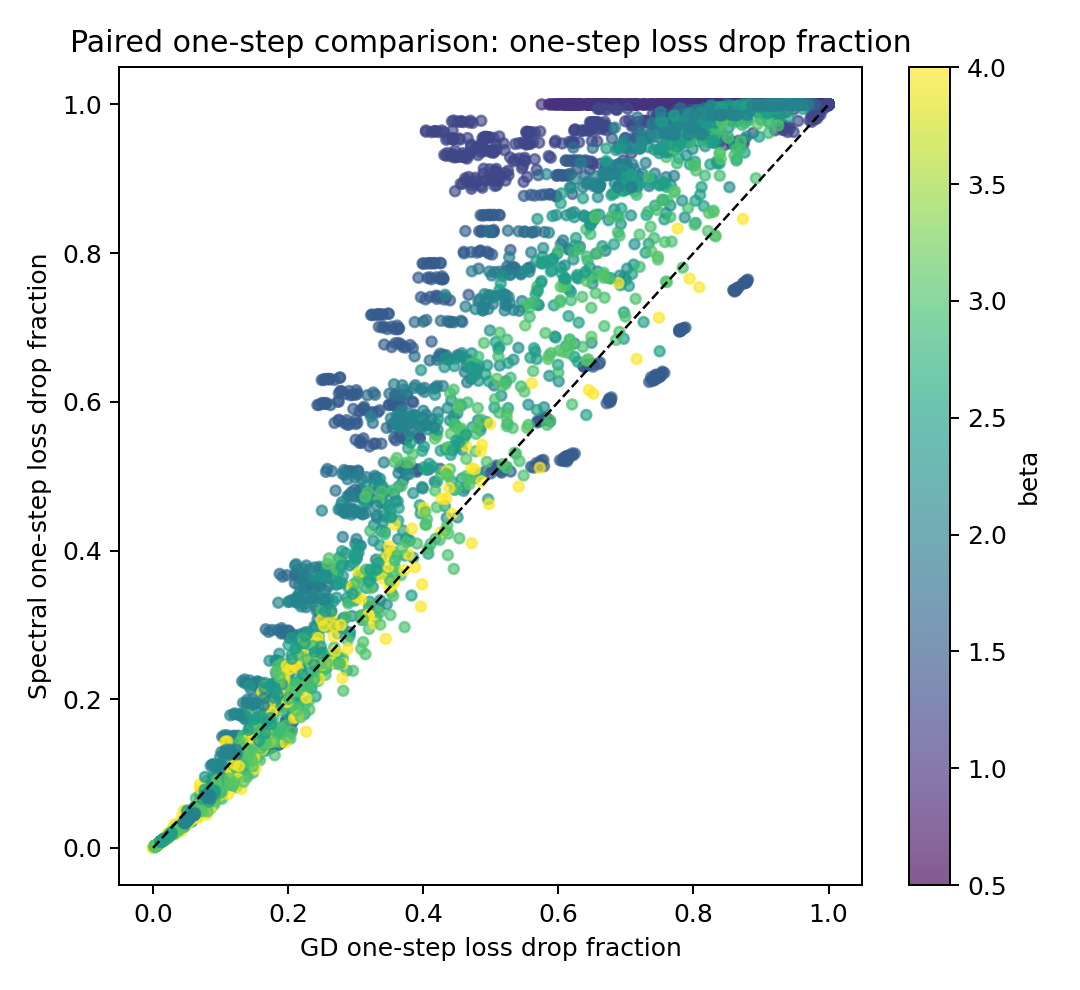
\includegraphics[width=\linewidth]{figures/paired_scatters/loss_drop_fraction.png}
  \caption{Loss-drop fraction}
\end{subfigure}
\hfill
\begin{subfigure}[t]{0.32\textwidth}
  \centering
  
\includegraphics[width=\linewidth]{figures/paired_scatters/unit_recovered_fraction.png}
  \caption{Hard count recovery}
\end{subfigure}
\caption{Experiment I paired instance-level comparison.  The first two panels
show the overall advantage of Muon/Spectral on task-relevant recovery and
loss reduction.  The hard-count panel is stricter and is most useful for
separating dominant-mass recovery from uniform recovery of all memories.}
\label{fig:exp1-paired-scatter-main}
\end{figure}

\subsection{Phase diagrams}

The following heatmaps use the largest exact-computable $d$ for each
$\beta$ block.  This choice makes the plots compact, but it should be read
together with Table~\ref{tab:grid-d-limits}: larger $\beta$ blocks have much
smaller available $d$.  Therefore the high-$\beta$ heatmap cells should be
viewed as conservative small-$d$ evidence.

\begin{figure}[H]
\centering
\begin{subfigure}[t]{0.32\textwidth}
  \centering
  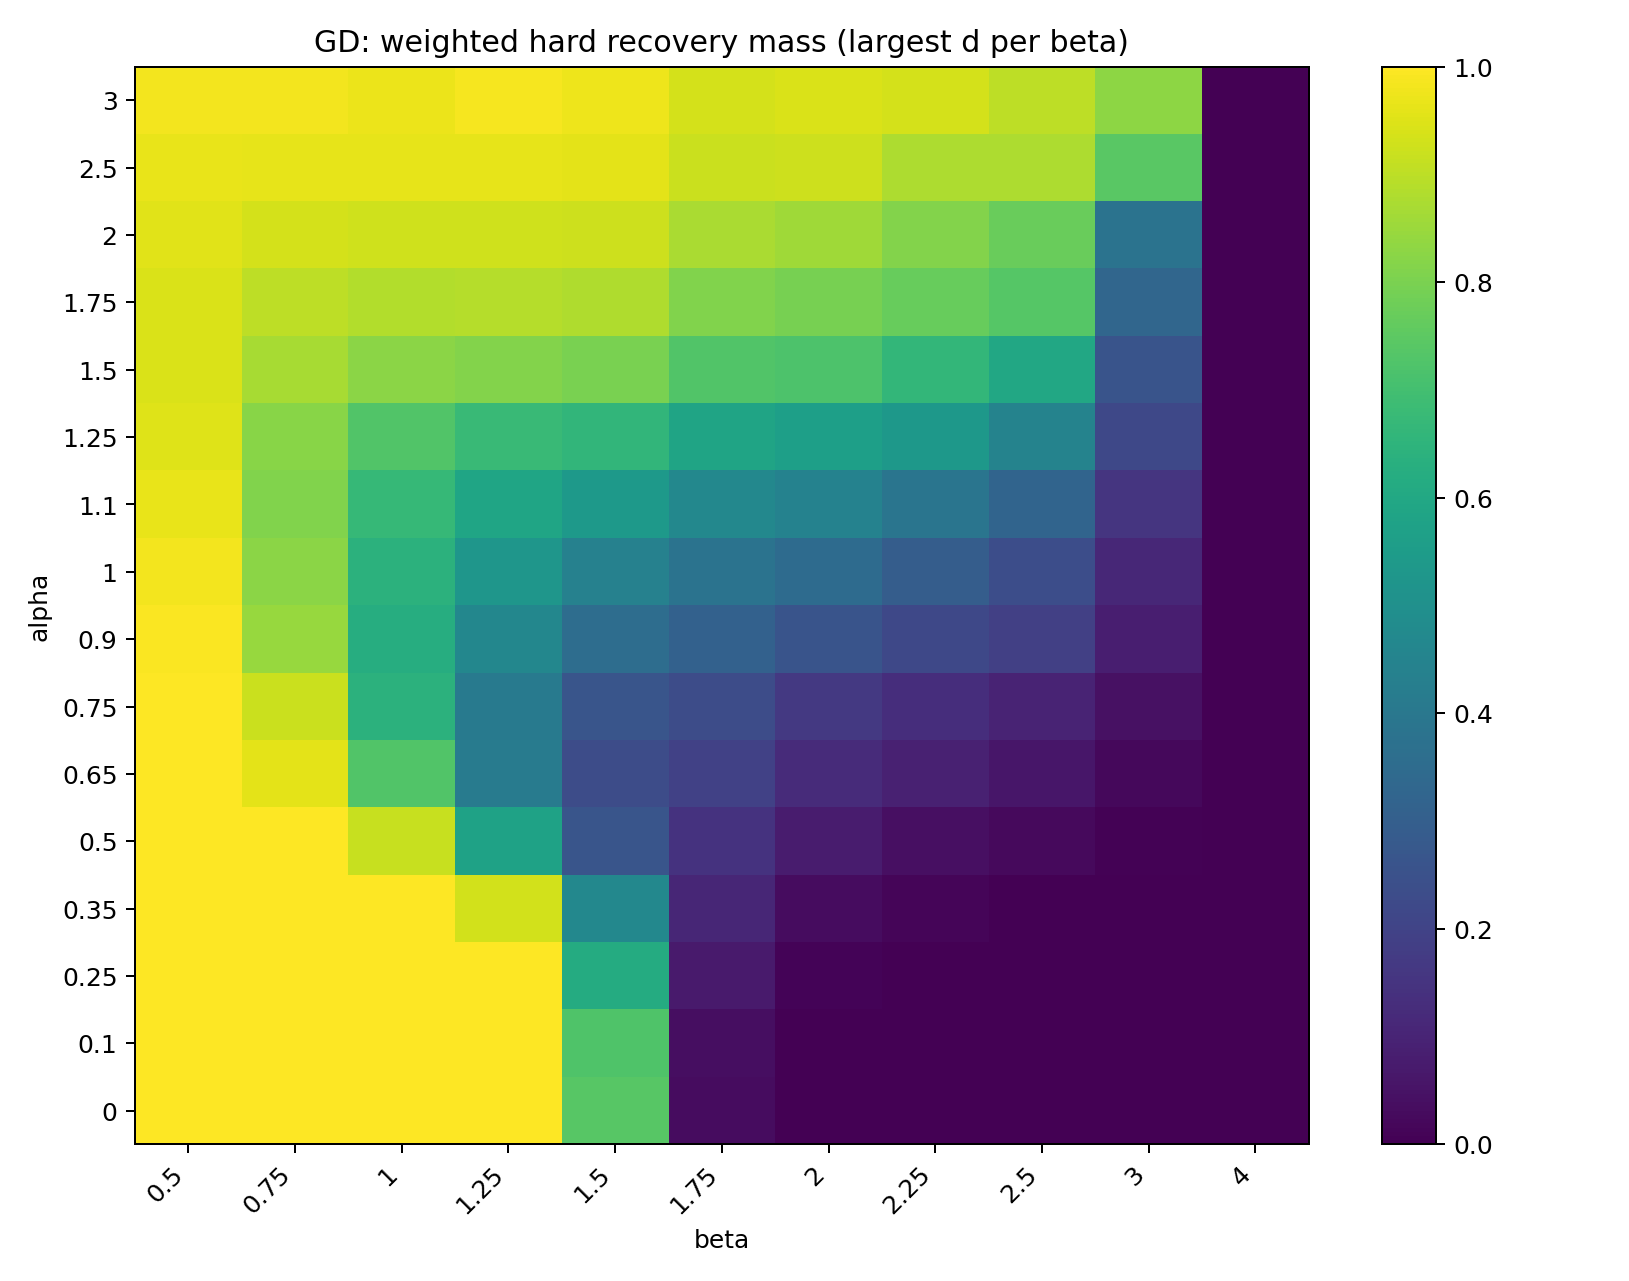
\includegraphics[width=\linewidth]{figures/heatmaps_largest_d/unit_weighted_recovered_mass_gd.png}
  \caption{GD}
\end{subfigure}
\hfill
\begin{subfigure}[t]{0.32\textwidth}
  \centering
  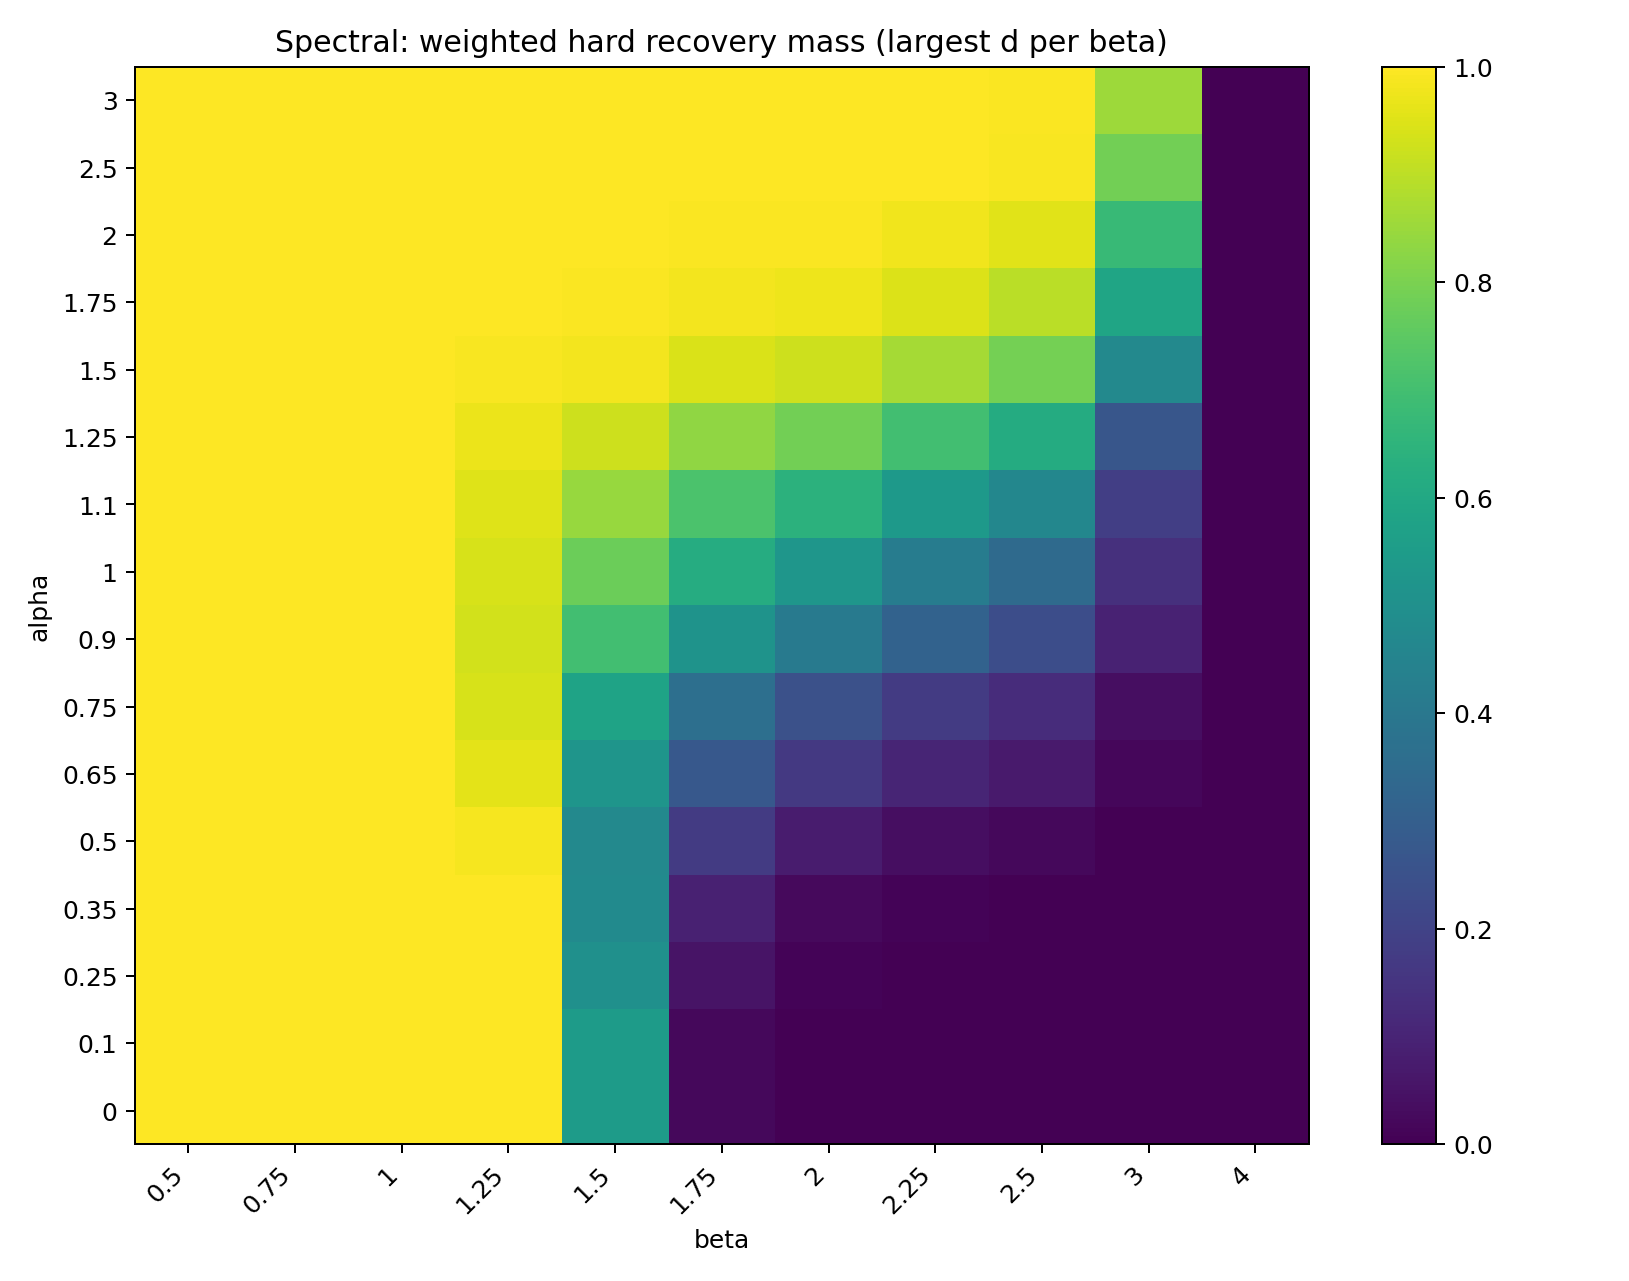
\includegraphics[width=\linewidth]{figures/heatmaps_largest_d/unit_weighted_recovered_mass_spectral.png}
  \caption{Muon/Spectral}
\end{subfigure}
\hfill
\begin{subfigure}[t]{0.32\textwidth}
  \centering
  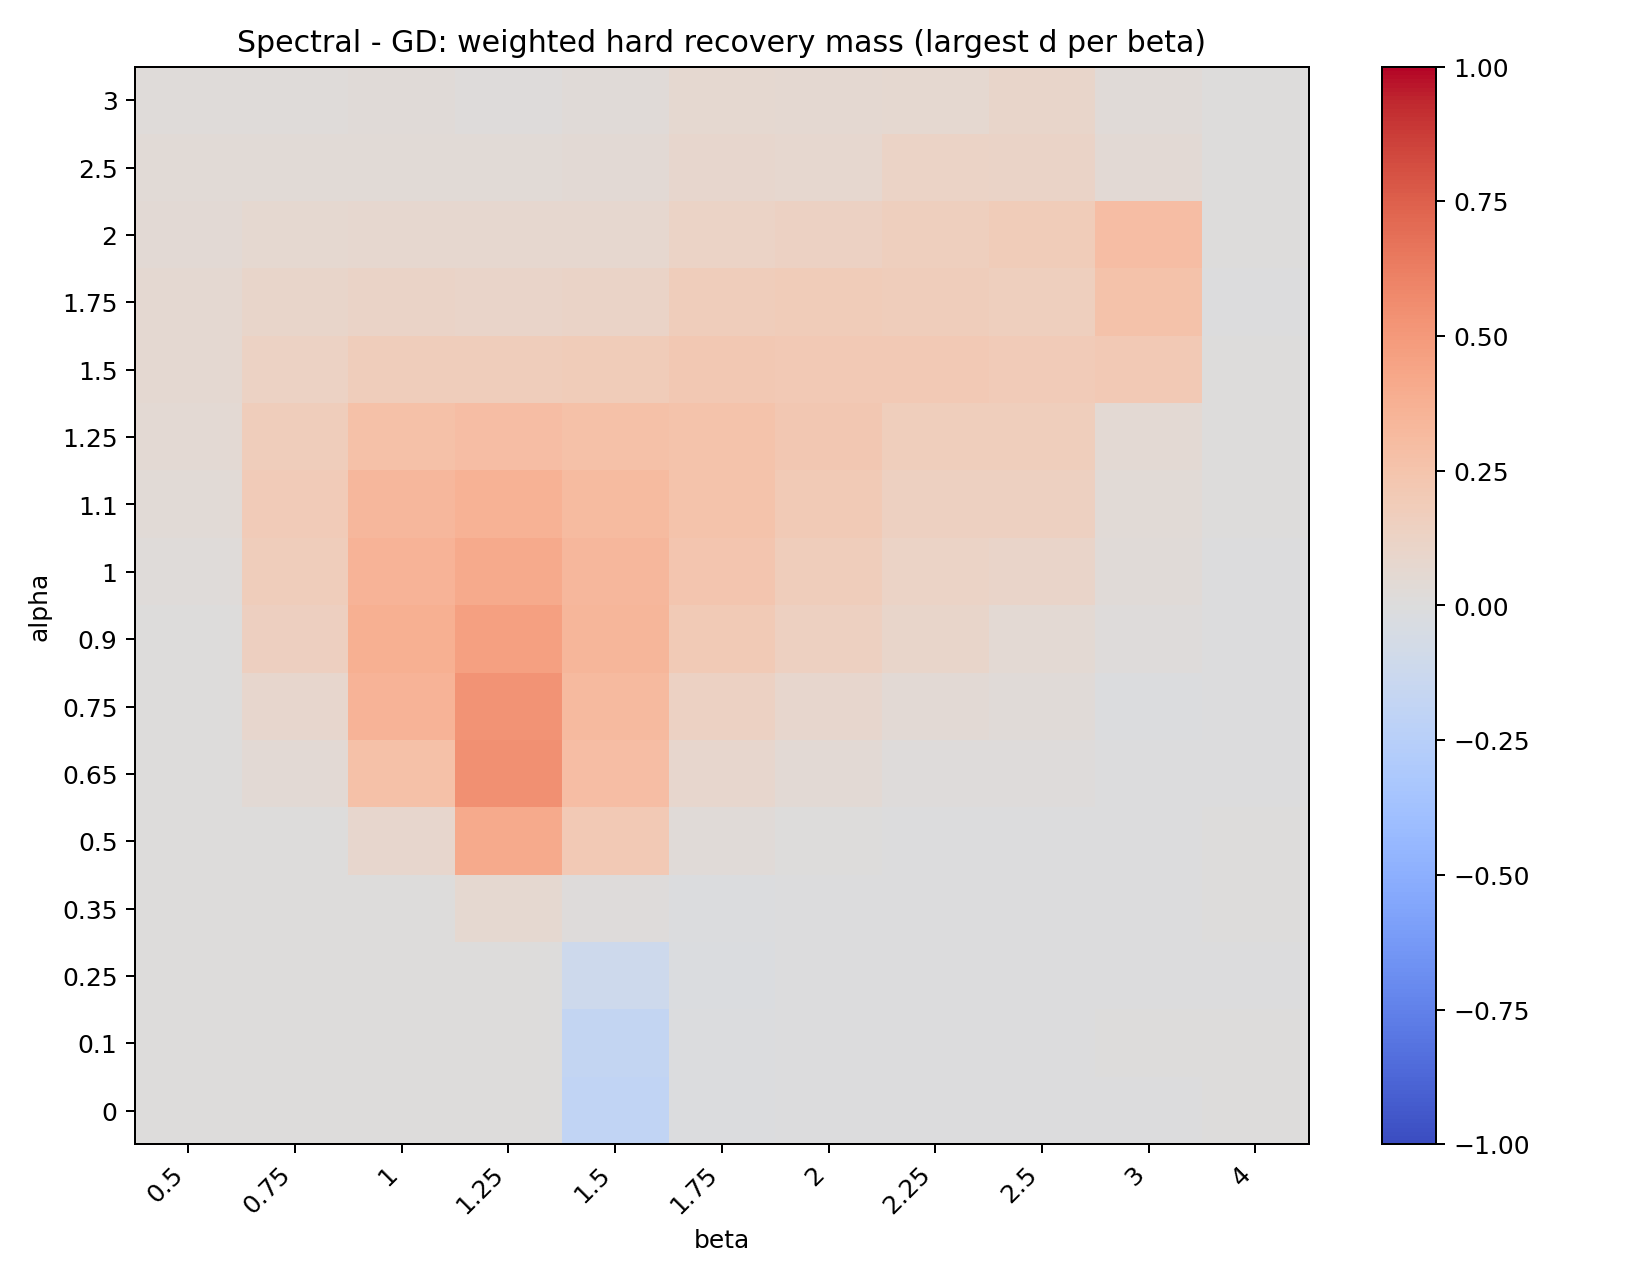
\includegraphics[width=\linewidth]{figures/heatmaps_largest_d/unit_weighted_recovered_mass_spectral_minus_gd.png}
  \caption{Muon $-$ GD}
\end{subfigure}
\caption{Experiment I weighted hard recovery.  This is the primary recovery
plot for the weighted associative-memory objective.  Muon/Spectral expands
the high-recovery region, especially around $\beta=1.5$--$2.5$ and
moderate-to-large $\alpha$.}
\label{fig:exp1-heatmap-weighted-recovery}
\end{figure}

\begin{figure}[H]
\centering
\begin{subfigure}[t]{0.32\textwidth}
  \centering
  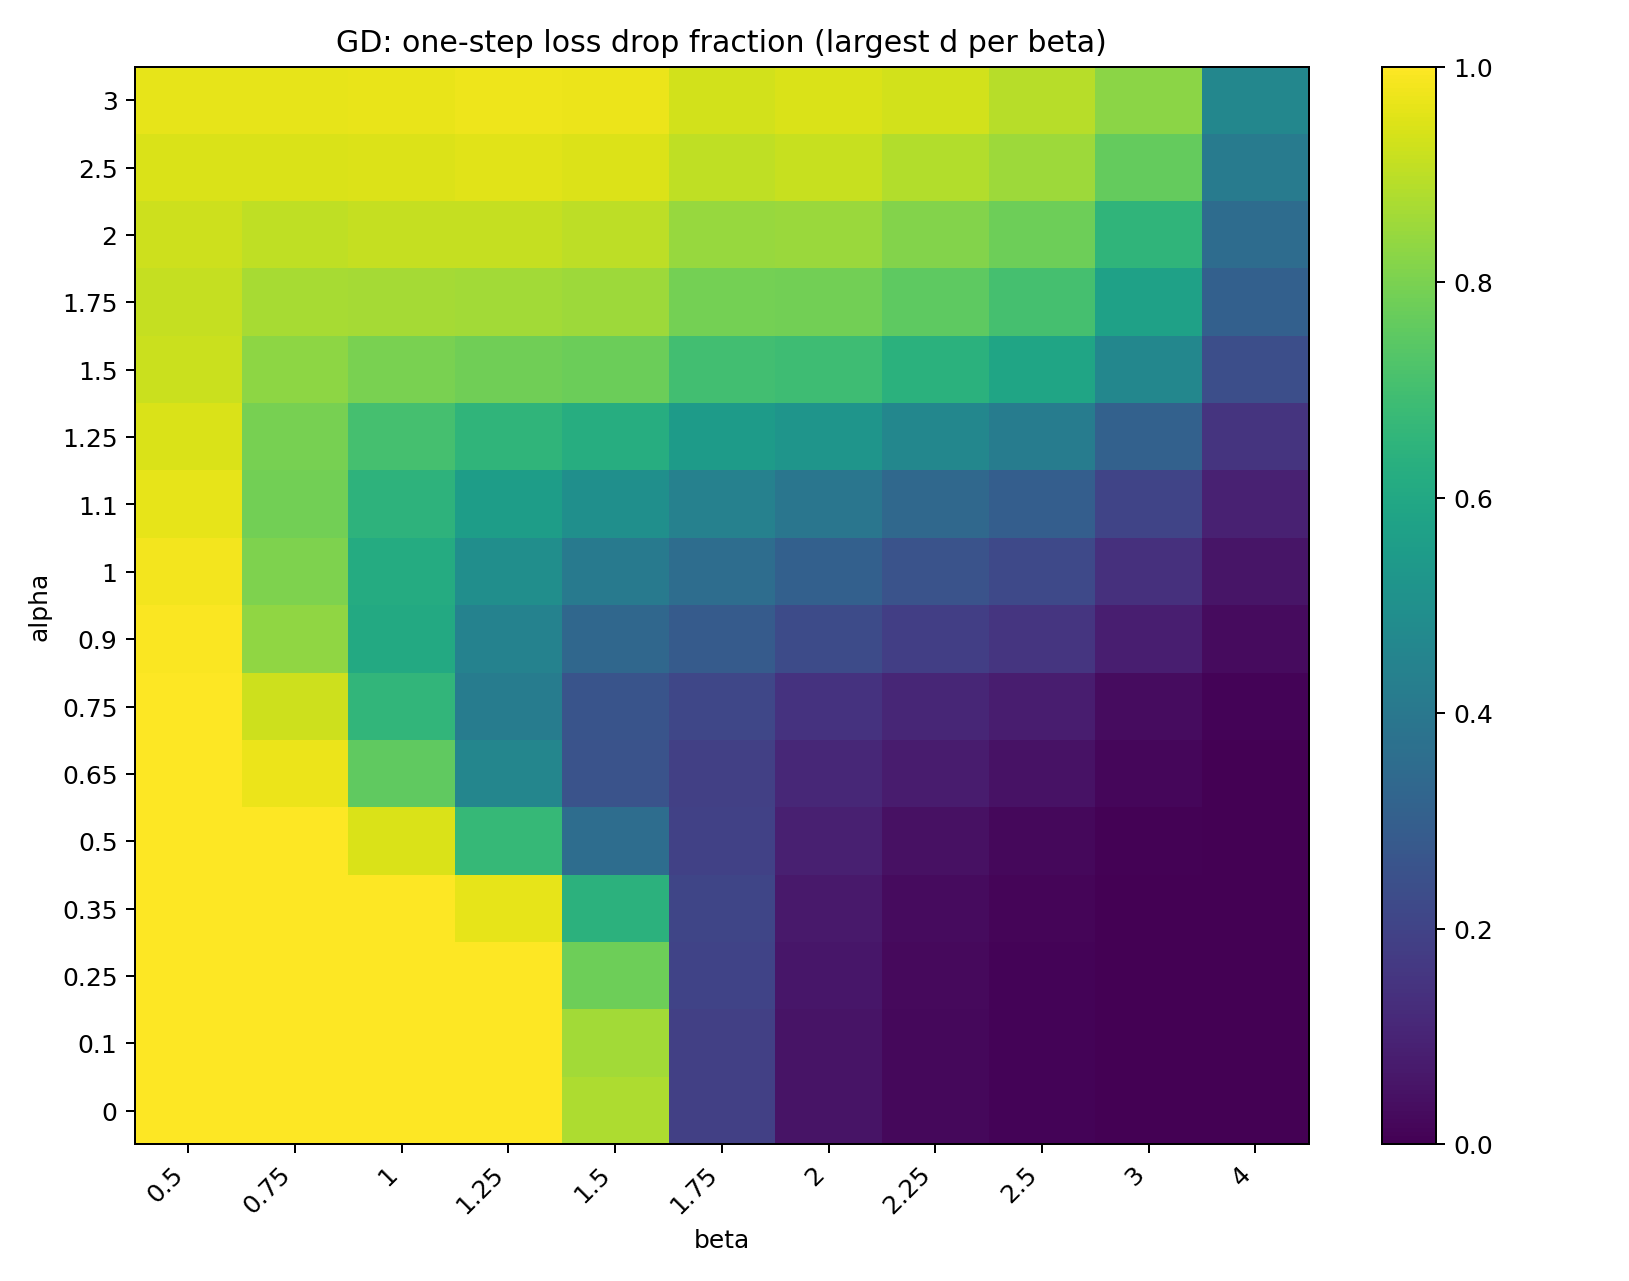
\includegraphics[width=\linewidth]{figures/heatmaps_largest_d/loss_drop_fraction_gd.png}
  \caption{GD}
\end{subfigure}
\hfill
\begin{subfigure}[t]{0.32\textwidth}
  \centering
  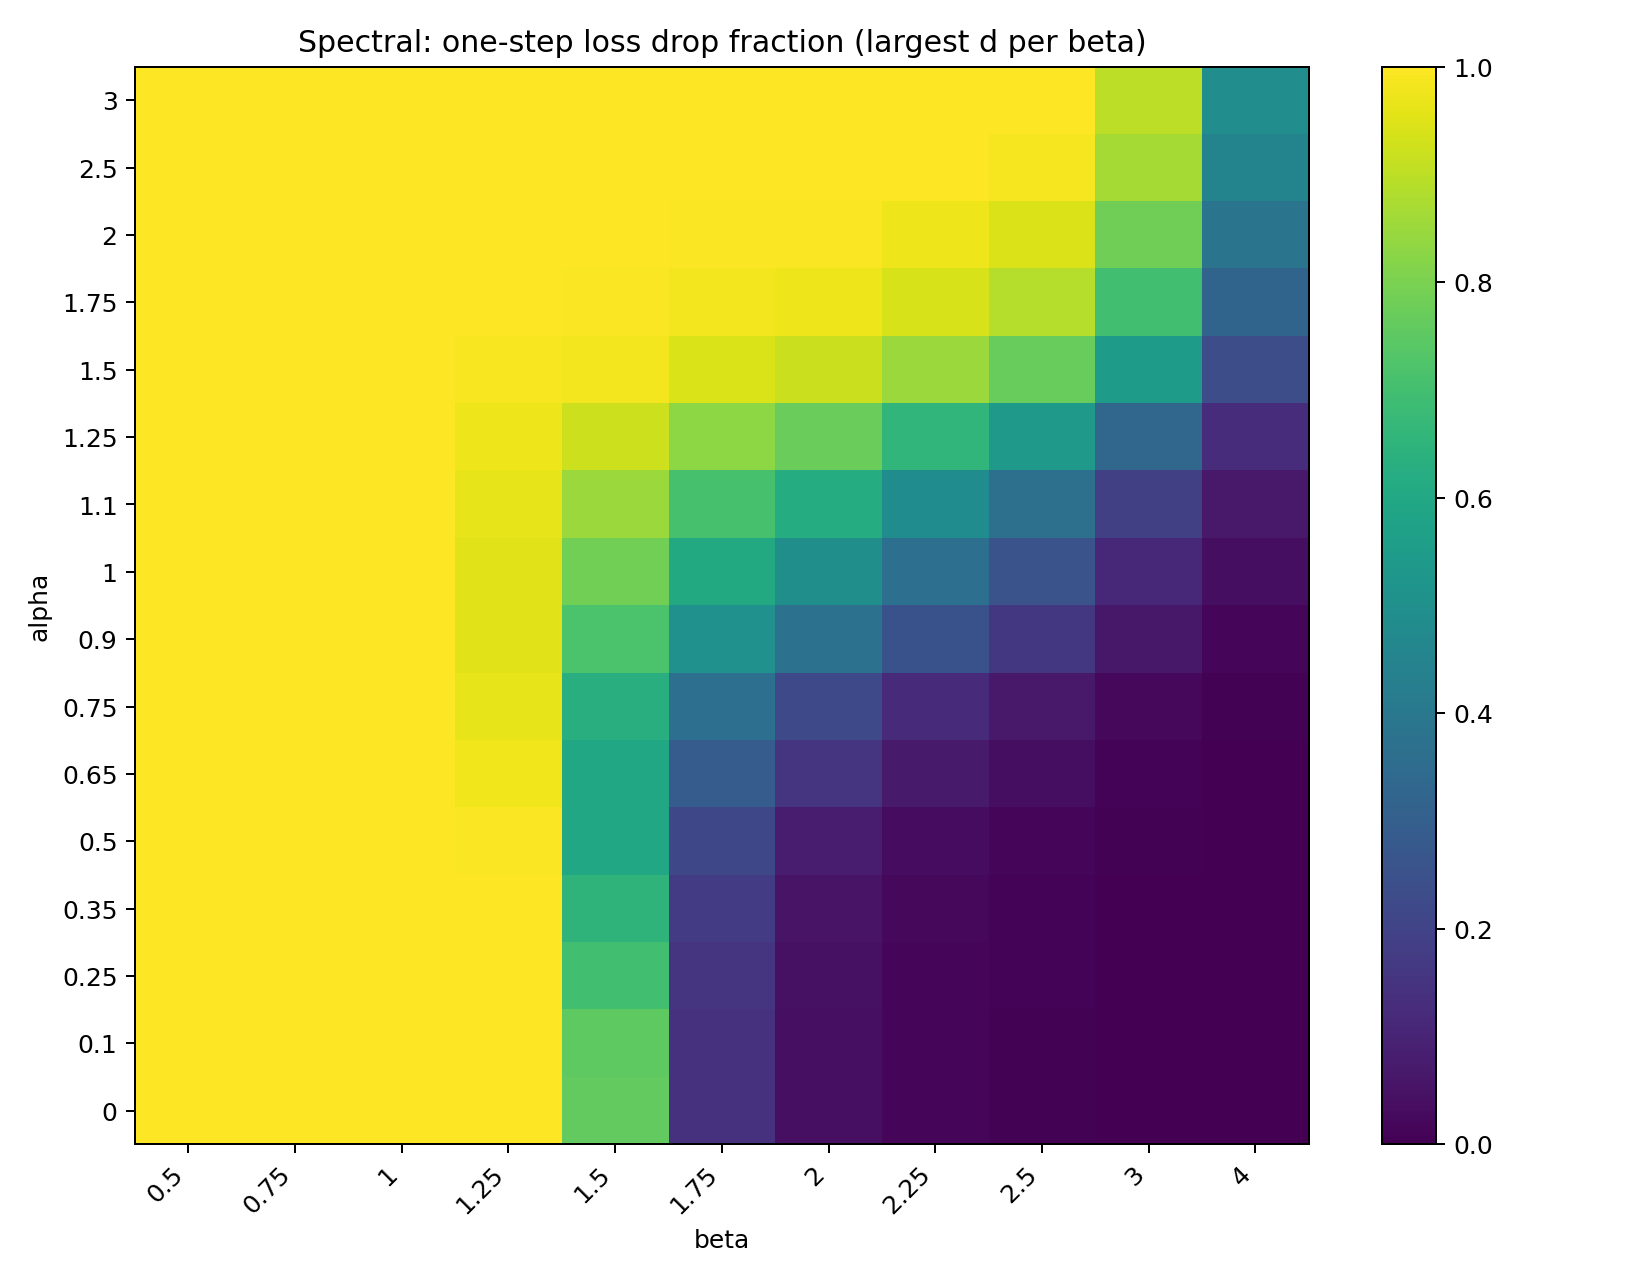
\includegraphics[width=\linewidth]{figures/heatmaps_largest_d/loss_drop_fraction_spectral.png}
  \caption{Muon/Spectral}
\end{subfigure}
\hfill
\begin{subfigure}[t]{0.32\textwidth}
  \centering
  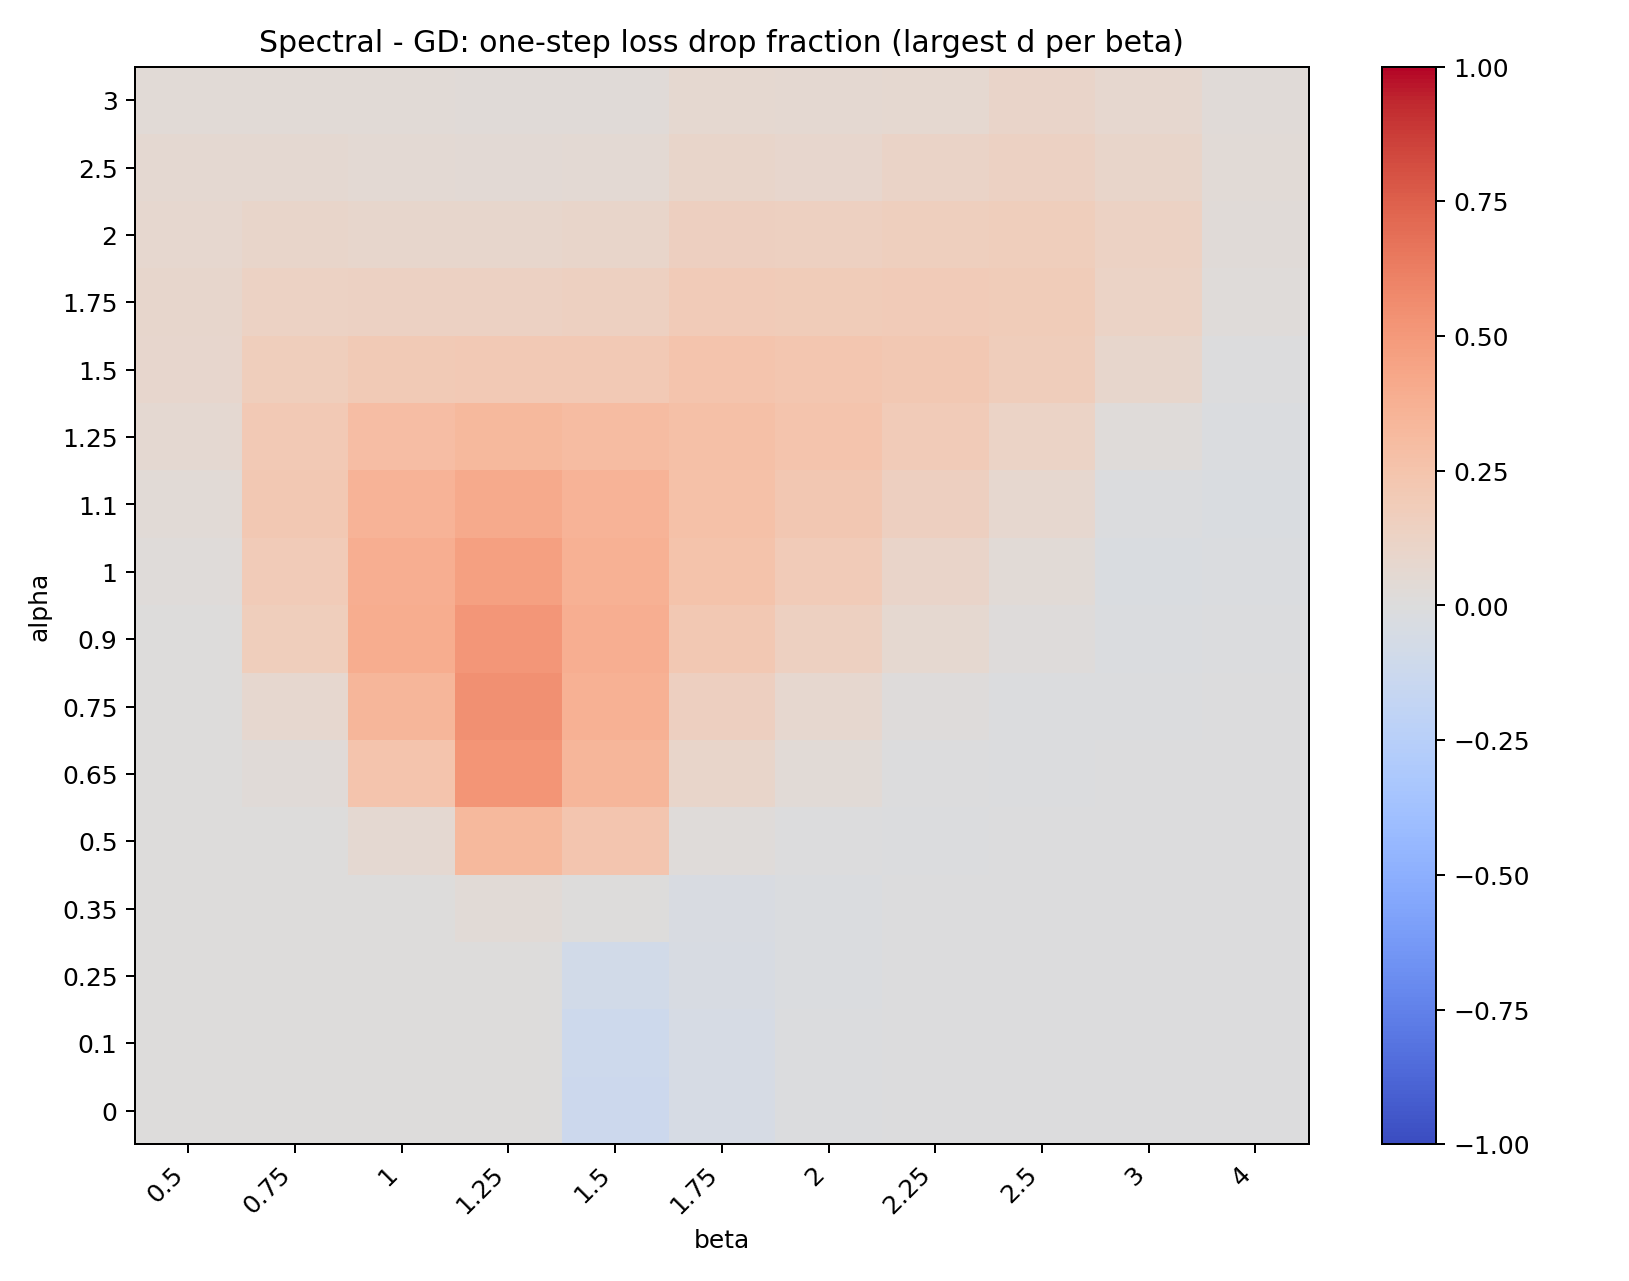
\includegraphics[width=\linewidth]{figures/heatmaps_largest_d/loss_drop_fraction_spectral_minus_gd.png}
  \caption{Muon $-$ GD}
\end{subfigure}
\caption{Experiment I one-step loss-drop fraction.  The loss metric confirms
that the recovery gains are accompanied by a large decrease in the actual
optimized objective.}
\label{fig:exp1-heatmap-loss-drop}
\end{figure}

\begin{figure}[H]
\centering
\begin{subfigure}[t]{0.32\textwidth}
  \centering
  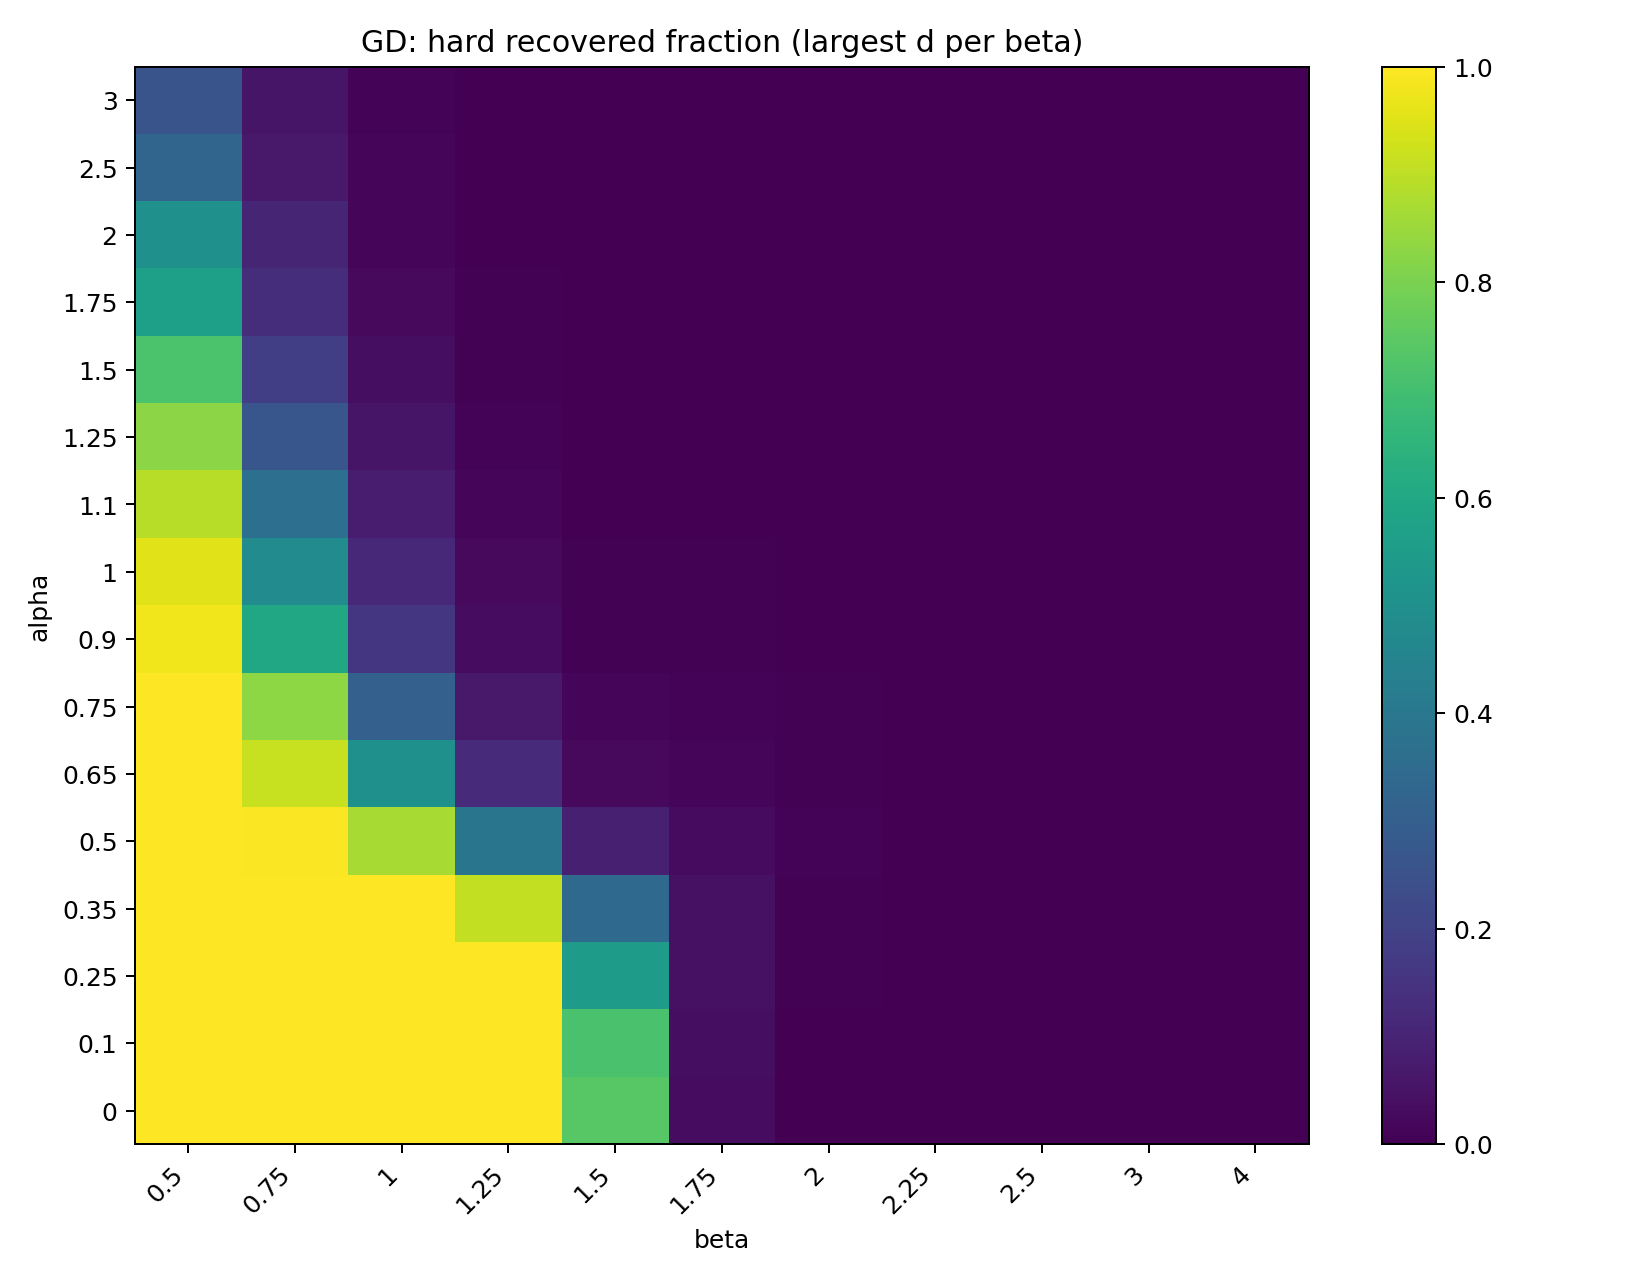
\includegraphics[width=\linewidth]{figures/heatmaps_largest_d/unit_recovered_fraction_gd.png}
  \caption{GD}
\end{subfigure}
\hfill
\begin{subfigure}[t]{0.32\textwidth}
  \centering
  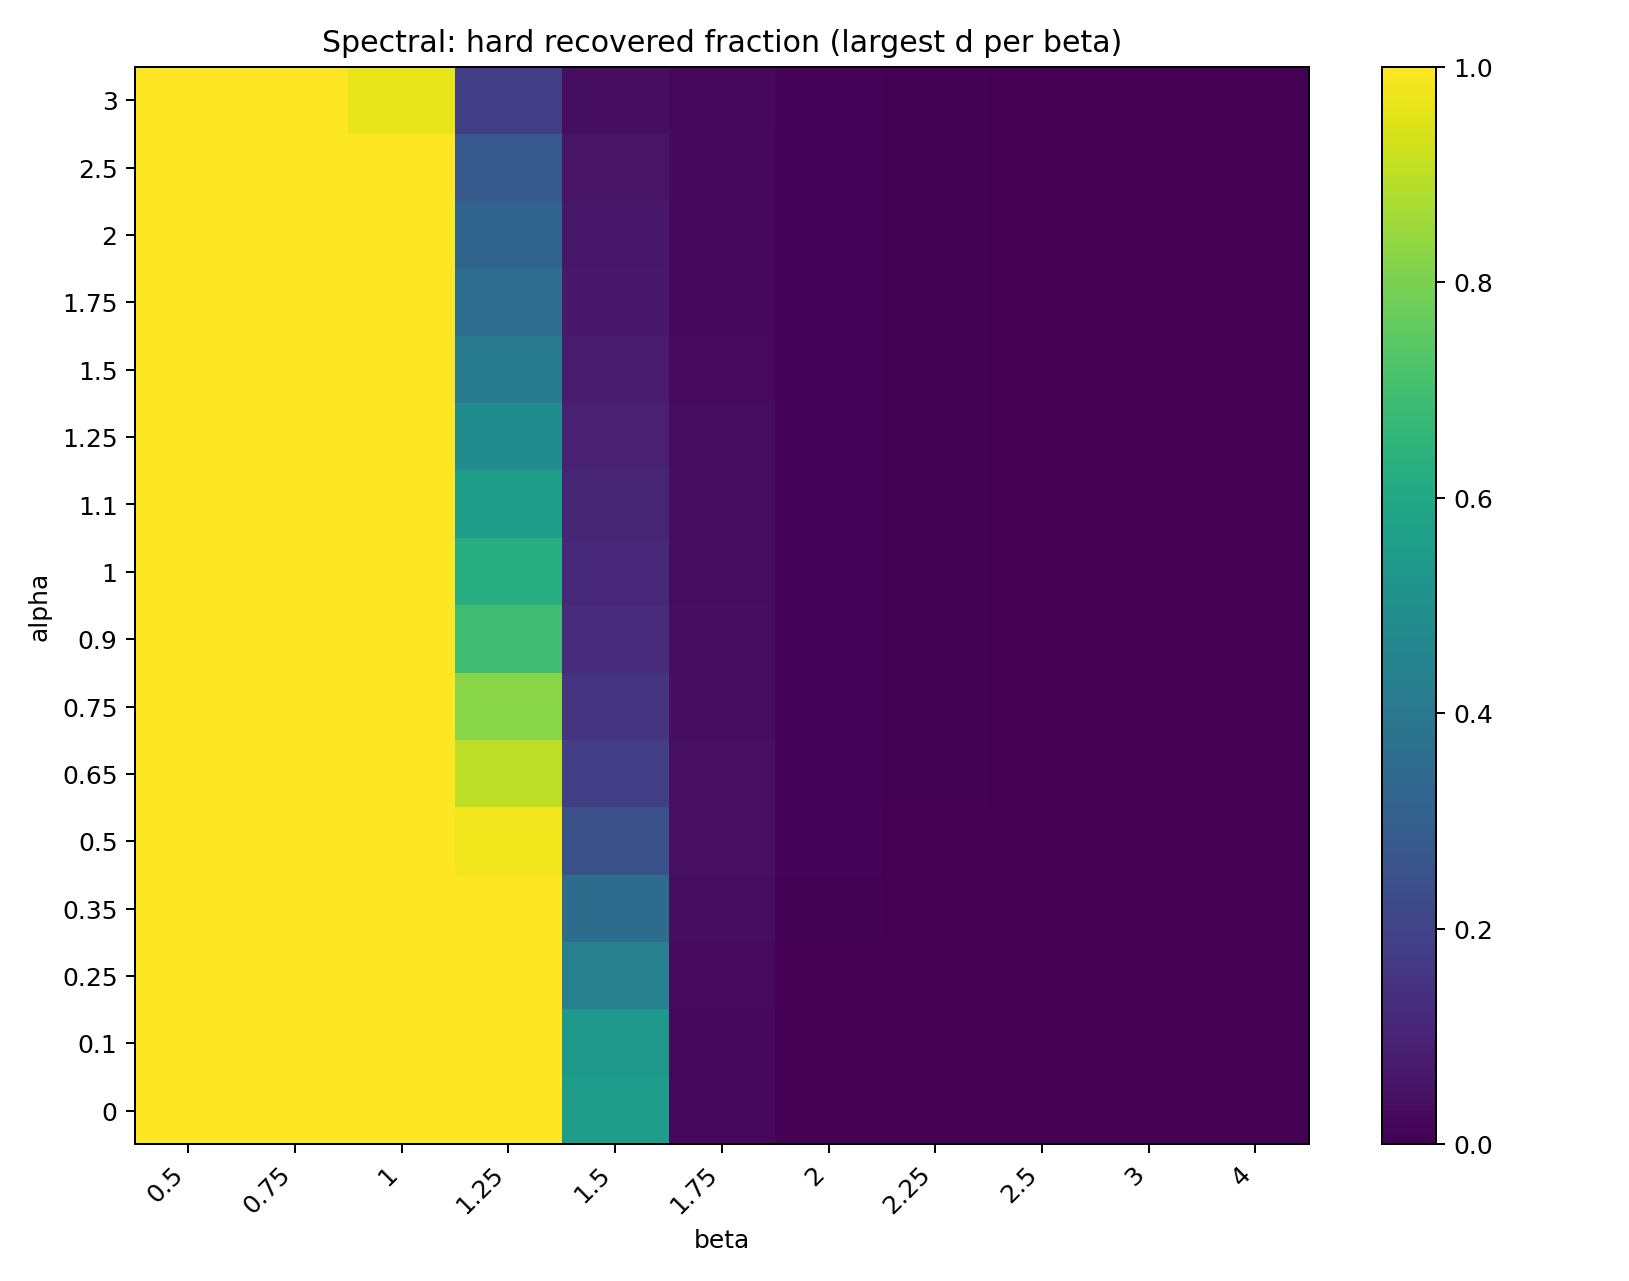
\includegraphics[width=\linewidth]{figures/heatmaps_largest_d/unit_recovered_fraction_spectral.png}
  \caption{Muon/Spectral}
\end{subfigure}
\hfill
\begin{subfigure}[t]{0.32\textwidth}
  \centering
  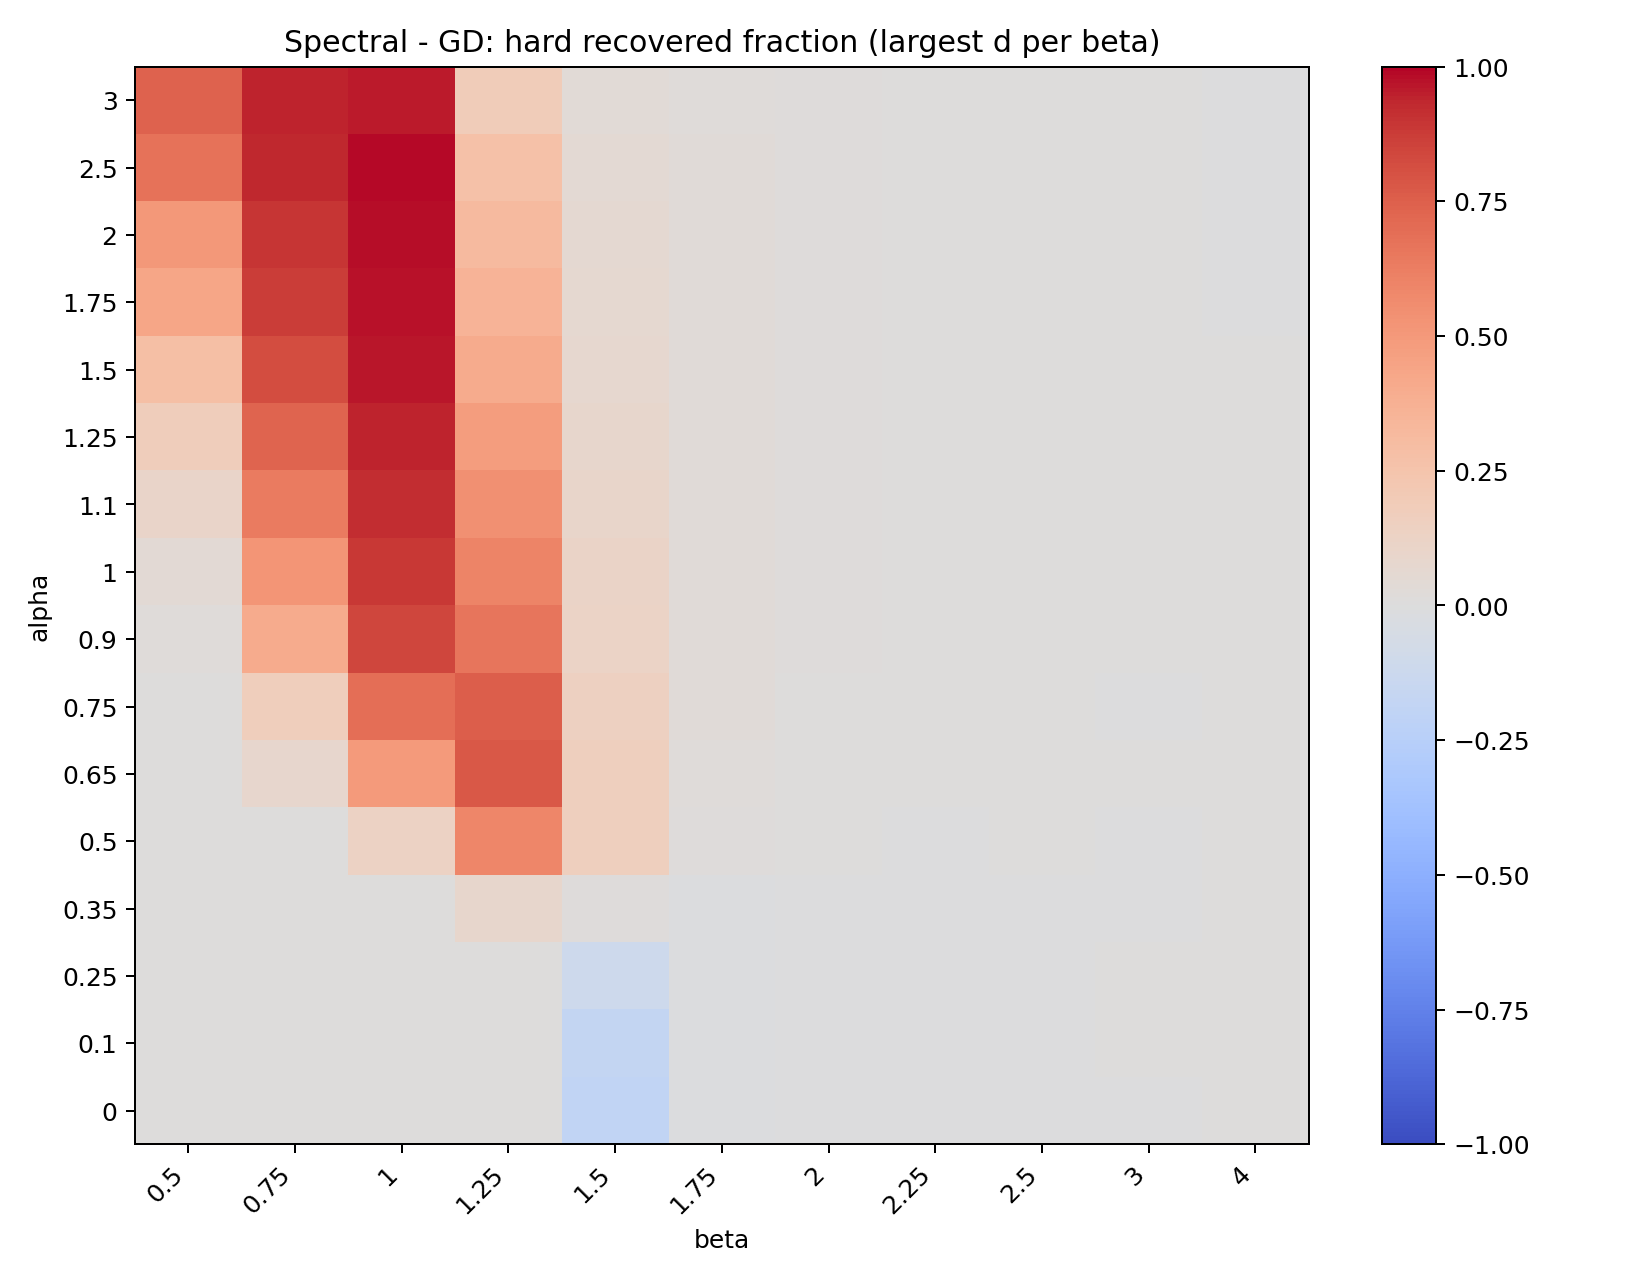
\includegraphics[width=\linewidth]{figures/heatmaps_largest_d/unit_recovered_fraction_spectral_minus_gd.png}
  \caption{Muon $-$ GD}
\end{subfigure}
\caption{Experiment I hard count recovery.  This is the strictest of the
three main metrics.  In large-$\beta$ regimes, count recovery is suppressed
both because the available $d$ is small and because $N$ can exceed the
natural $d^2$ recovery scale.}
\label{fig:exp1-heatmap-count-recovery}
\end{figure}

\subsection{Large-beta interpretation for Experiment I}

The Experiment~I heatmaps should not be presented as a full verification of
the recovery theory for every $\beta<2$.  The obstacle is computational:
exact all-pairs evaluation requires $N^2$ logits, and for $N=d^\beta$ this
becomes prohibitive precisely when $\beta$ is large.  As a result, the
largest-$\beta$ blocks use much smaller dimensions than the low-$\beta$
blocks.  Since the predicted recovery improves as $d$ grows, low-alpha
weakness in these large-$\beta$ exact plots is best interpreted as a
conservative consequence of insufficiently large $d$.

\section{Experiment II results: one step versus convergence reference}

\subsection{Instance-level fractions}

Figure~\ref{fig:exp2-one-vs-conv-scatter} plots one-step outcomes against
the convergence reference.  Points near the diagonal mean that one step
already matches the reference optimizer on that metric.

\begin{figure}[H]
\centering
\begin{subfigure}[t]{0.32\textwidth}
  \centering
  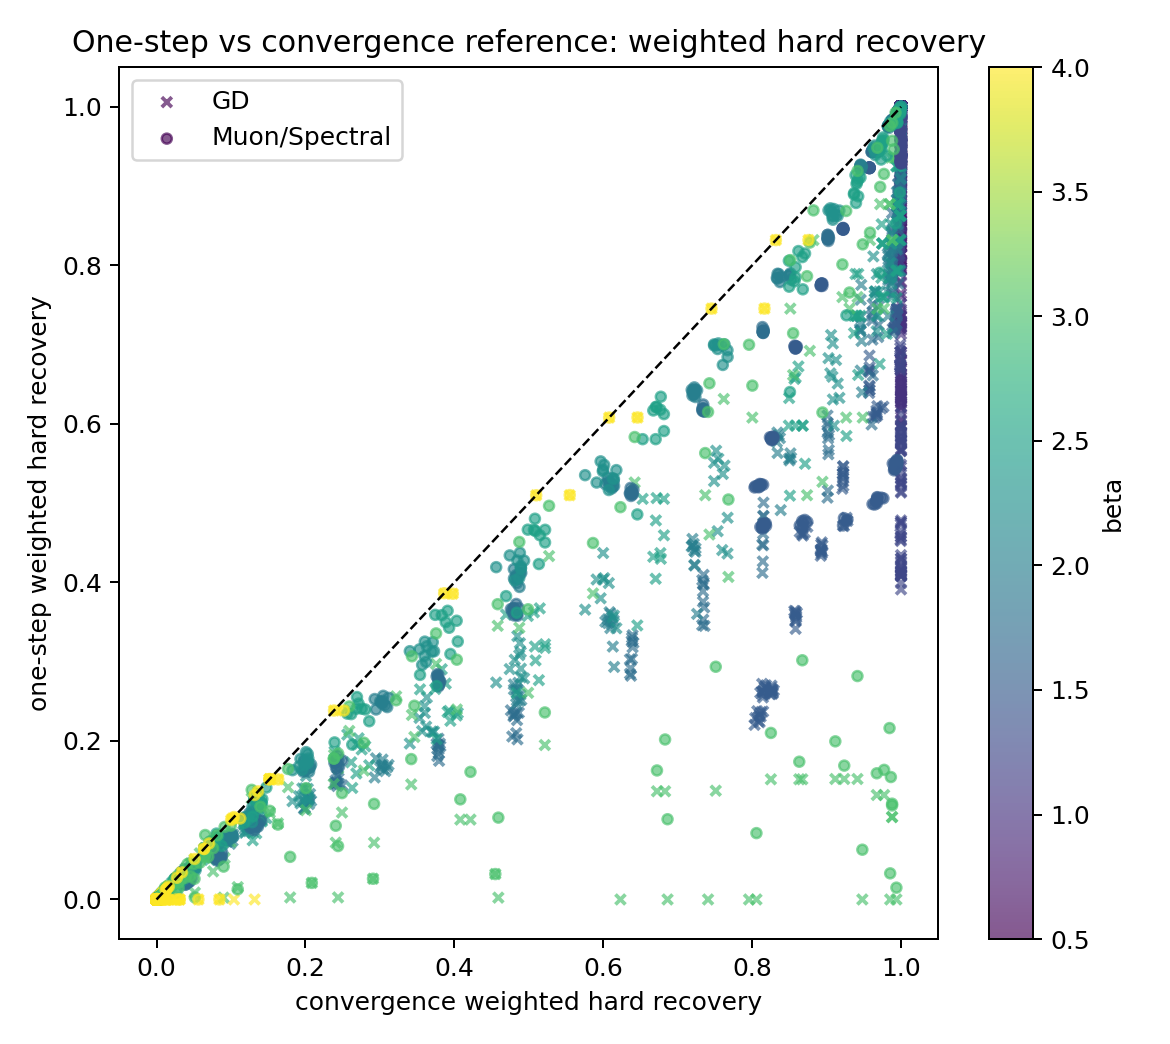
\includegraphics[width=\linewidth]{figures/one_step_vs_convergence/unit_weighted_recovered_mass.png}
  \caption{Weighted hard recovery}
\end{subfigure}
\hfill
\begin{subfigure}[t]{0.32\textwidth}
  \centering
  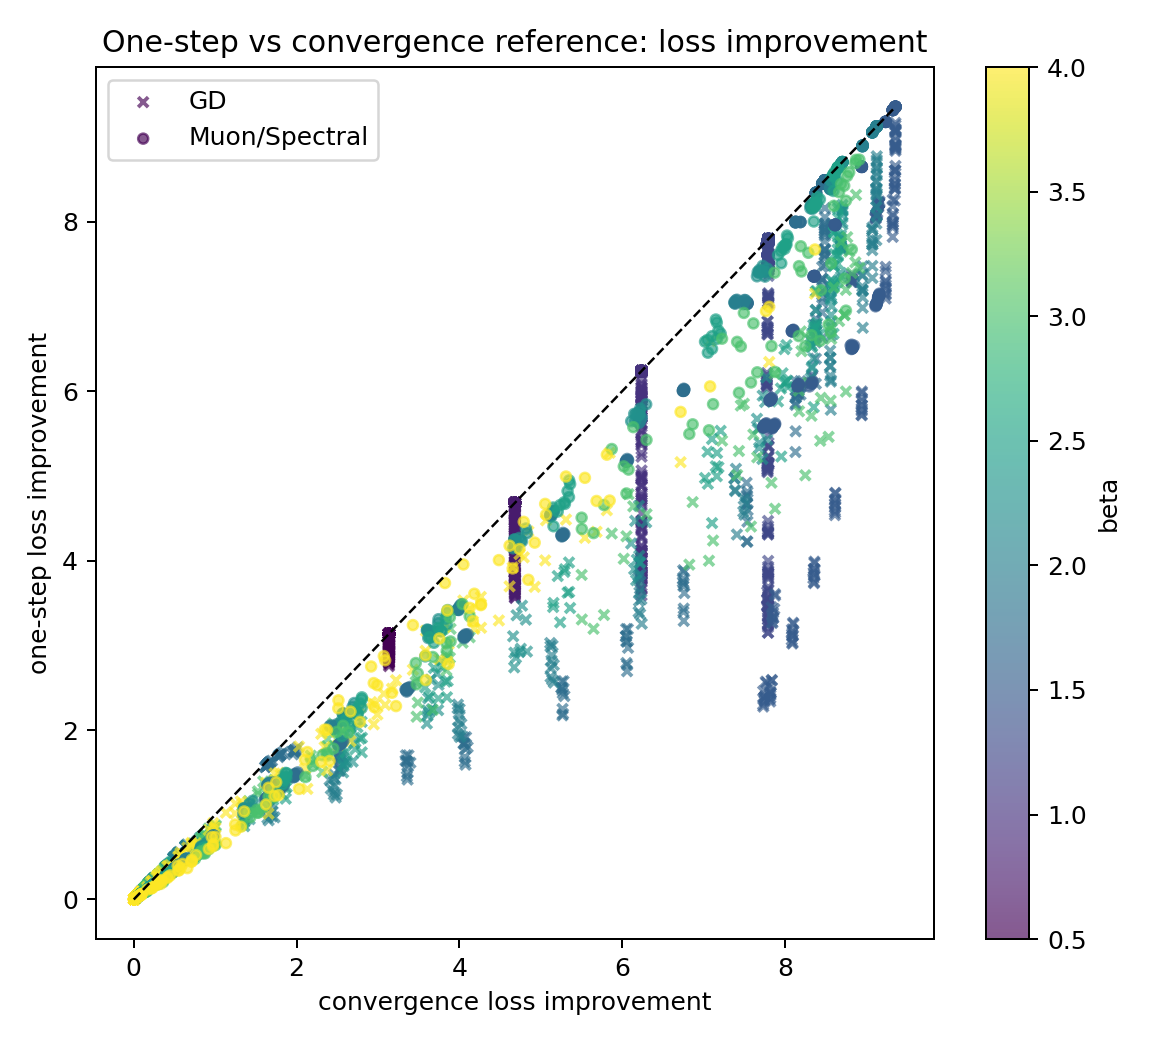
\includegraphics[width=\linewidth]{figures/one_step_vs_convergence/loss_improvement.png}
  \caption{Loss improvement}
\end{subfigure}
\hfill
\begin{subfigure}[t]{0.32\textwidth}
  \centering
  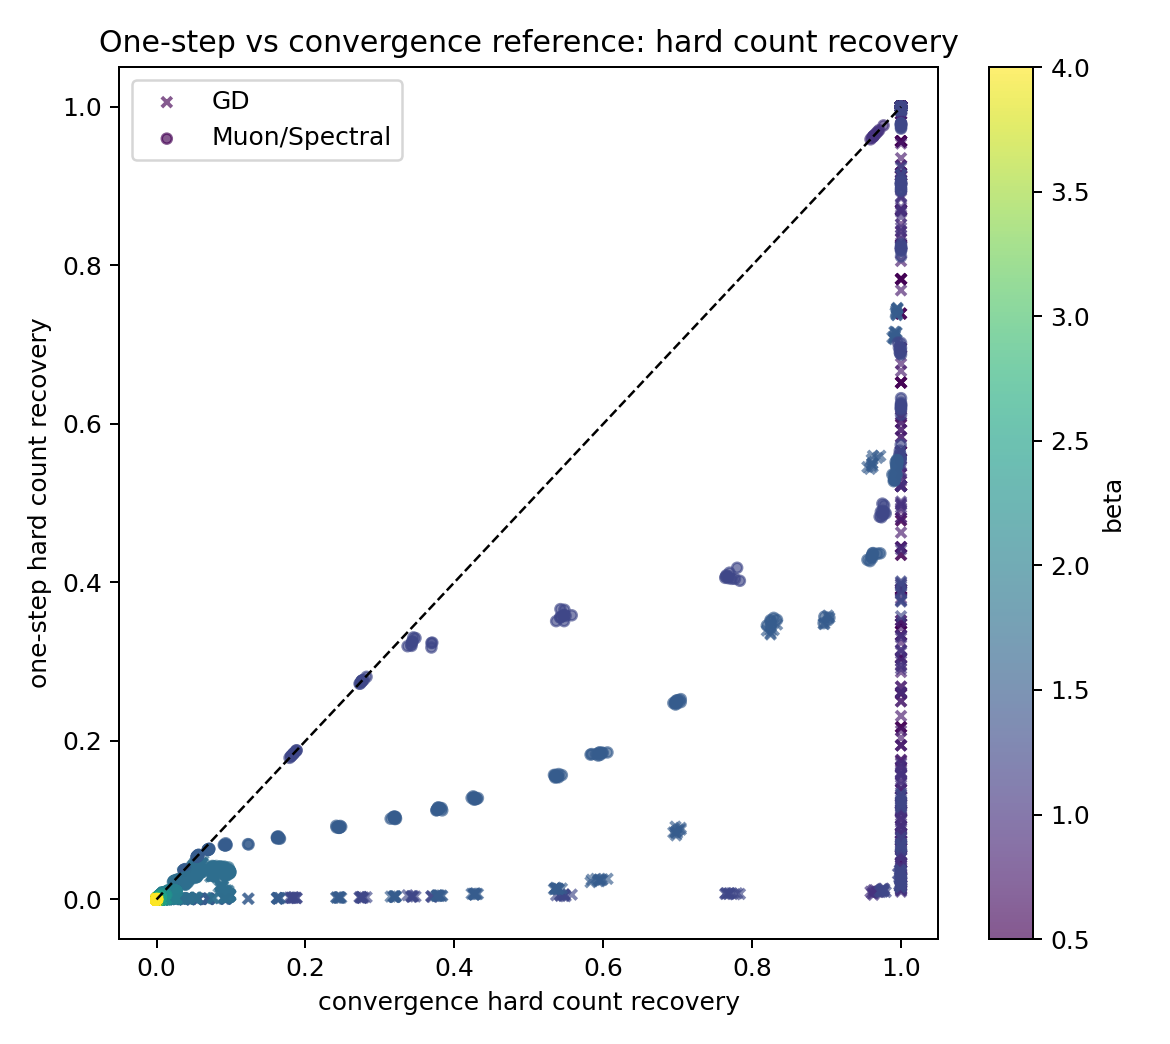
\includegraphics[width=\linewidth]{figures/one_step_vs_convergence/unit_recovered_fraction.png}
  \caption{Hard count recovery}
\end{subfigure}
\caption{Experiment II instance-level comparison between the best one-step
update and the convergence reference.  The diagonal is equality.  Colors
indicate $\beta$ and marker shape distinguishes GD from Muon/Spectral.}
\label{fig:exp2-one-vs-conv-scatter}
\end{figure}

\subsection{Fraction heatmaps}

The next heatmaps summarize the seed-median one-step fraction of the
convergence reference at the largest feasible $d$ for each $\beta$.  The
difference panel is Muon/Spectral minus GD.

\begin{figure}[H]
\centering
\begin{subfigure}[t]{0.32\textwidth}
  \centering
  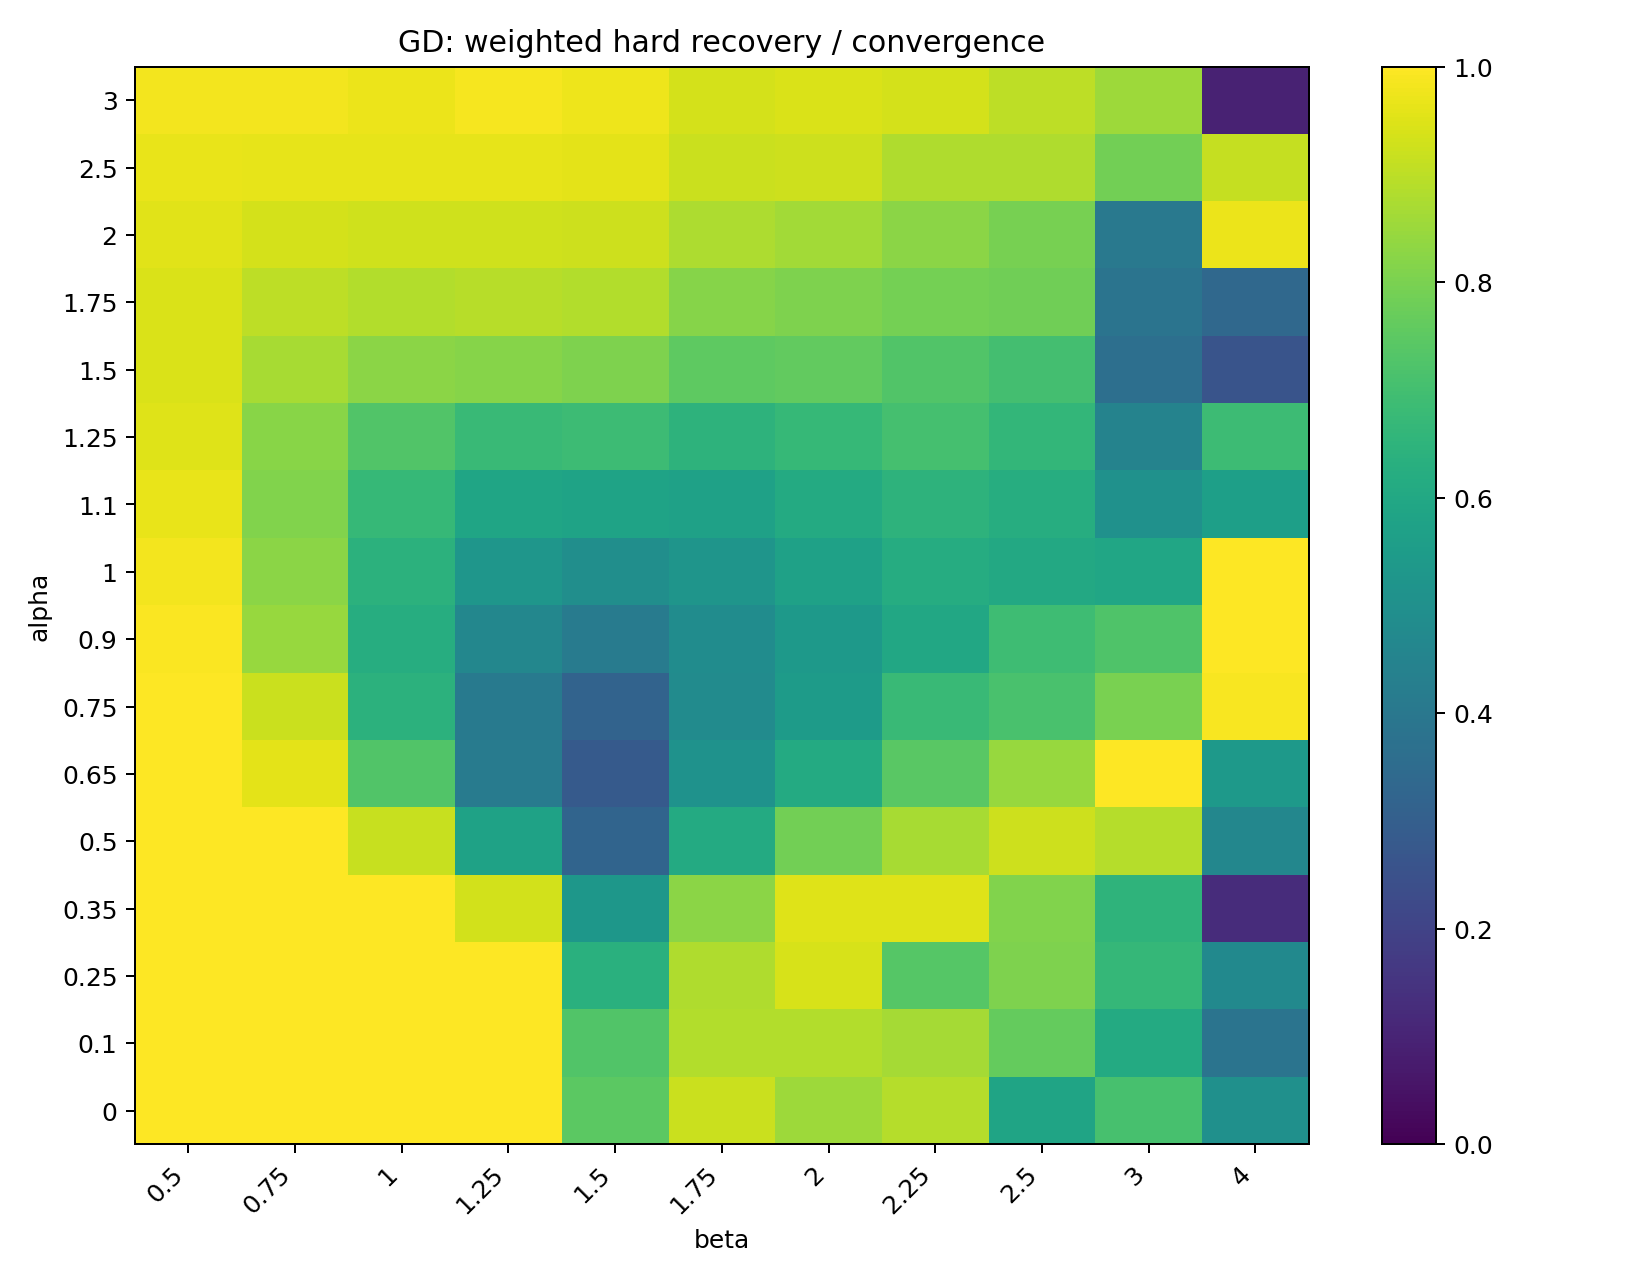
\includegraphics[width=\linewidth]{figures/fraction_heatmaps/unit_weighted_recovered_mass_fraction_gd.png}
  \caption{GD}
\end{subfigure}
\hfill
\begin{subfigure}[t]{0.32\textwidth}
  \centering
  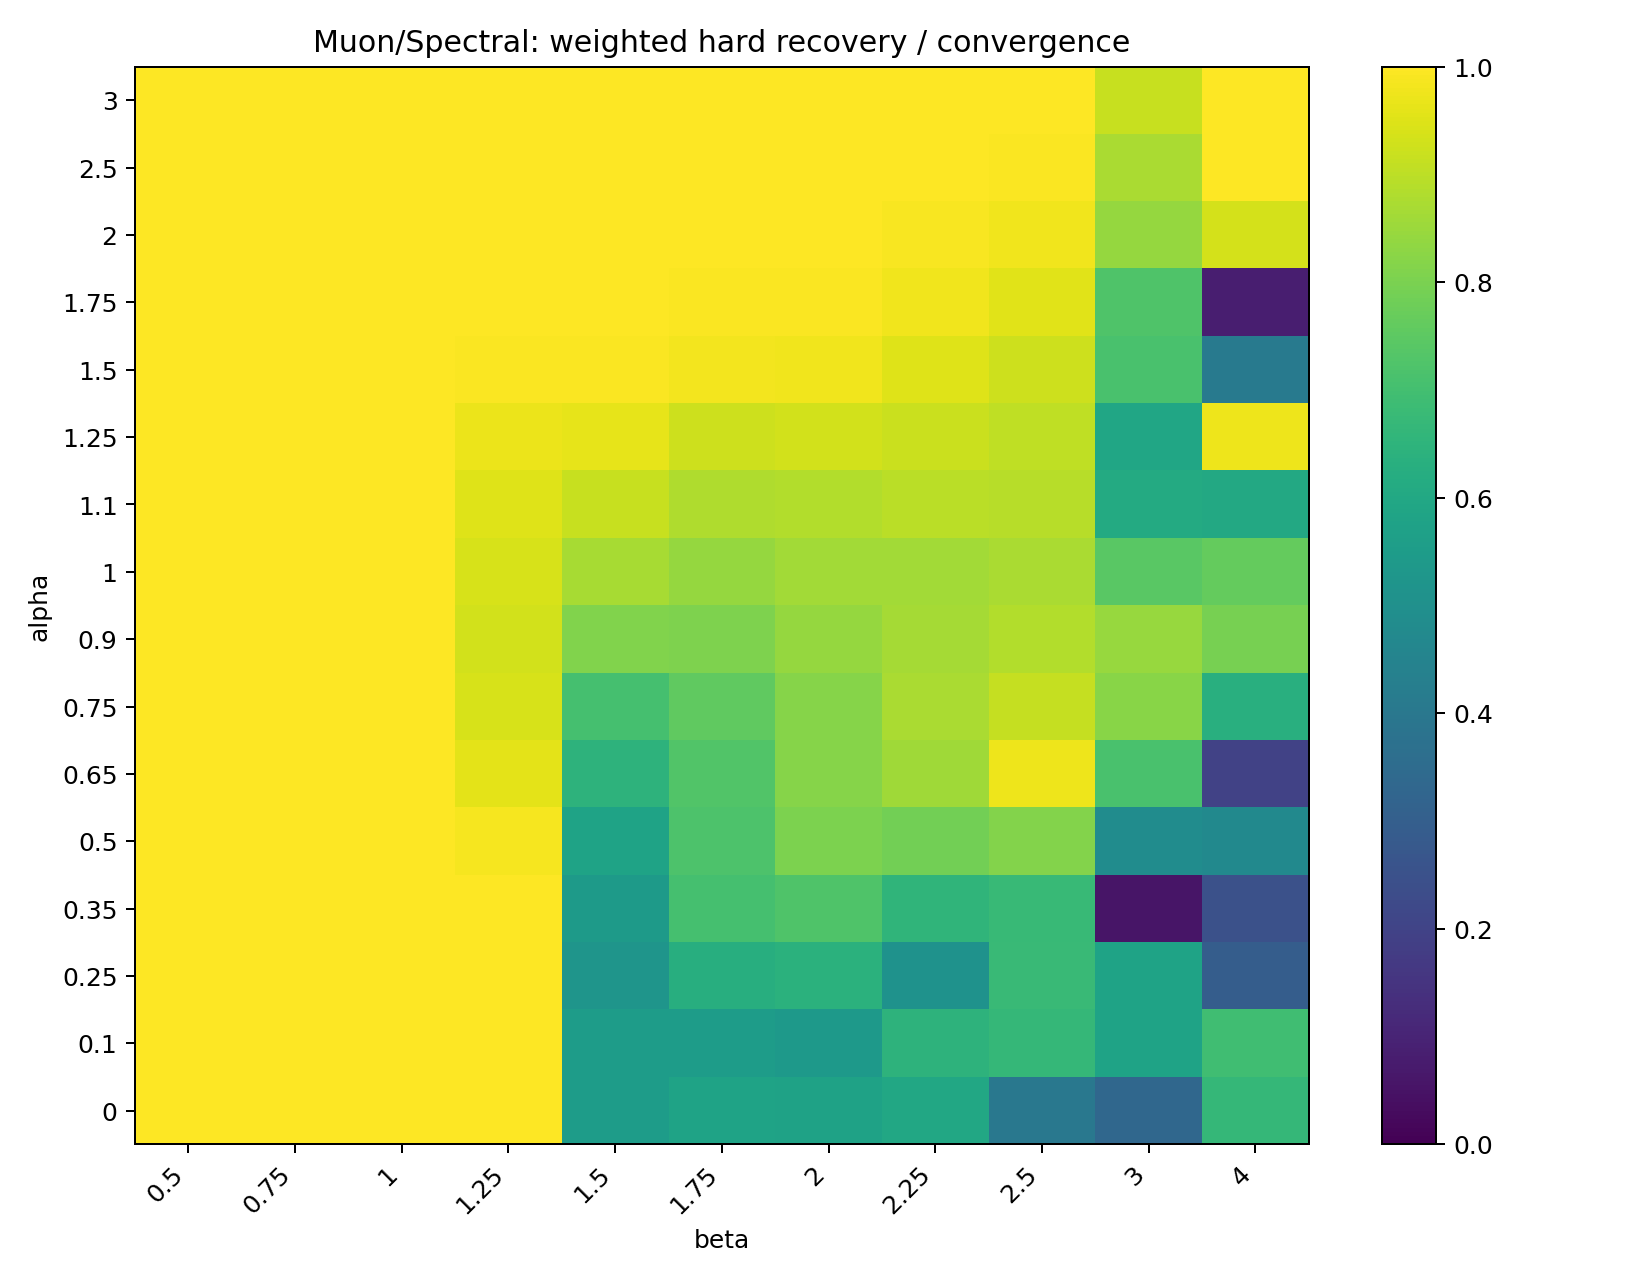
\includegraphics[width=\linewidth]{figures/fraction_heatmaps/unit_weighted_recovered_mass_fraction_spectral.png}
  \caption{Muon/Spectral}
\end{subfigure}
\hfill
\begin{subfigure}[t]{0.32\textwidth}
  \centering
  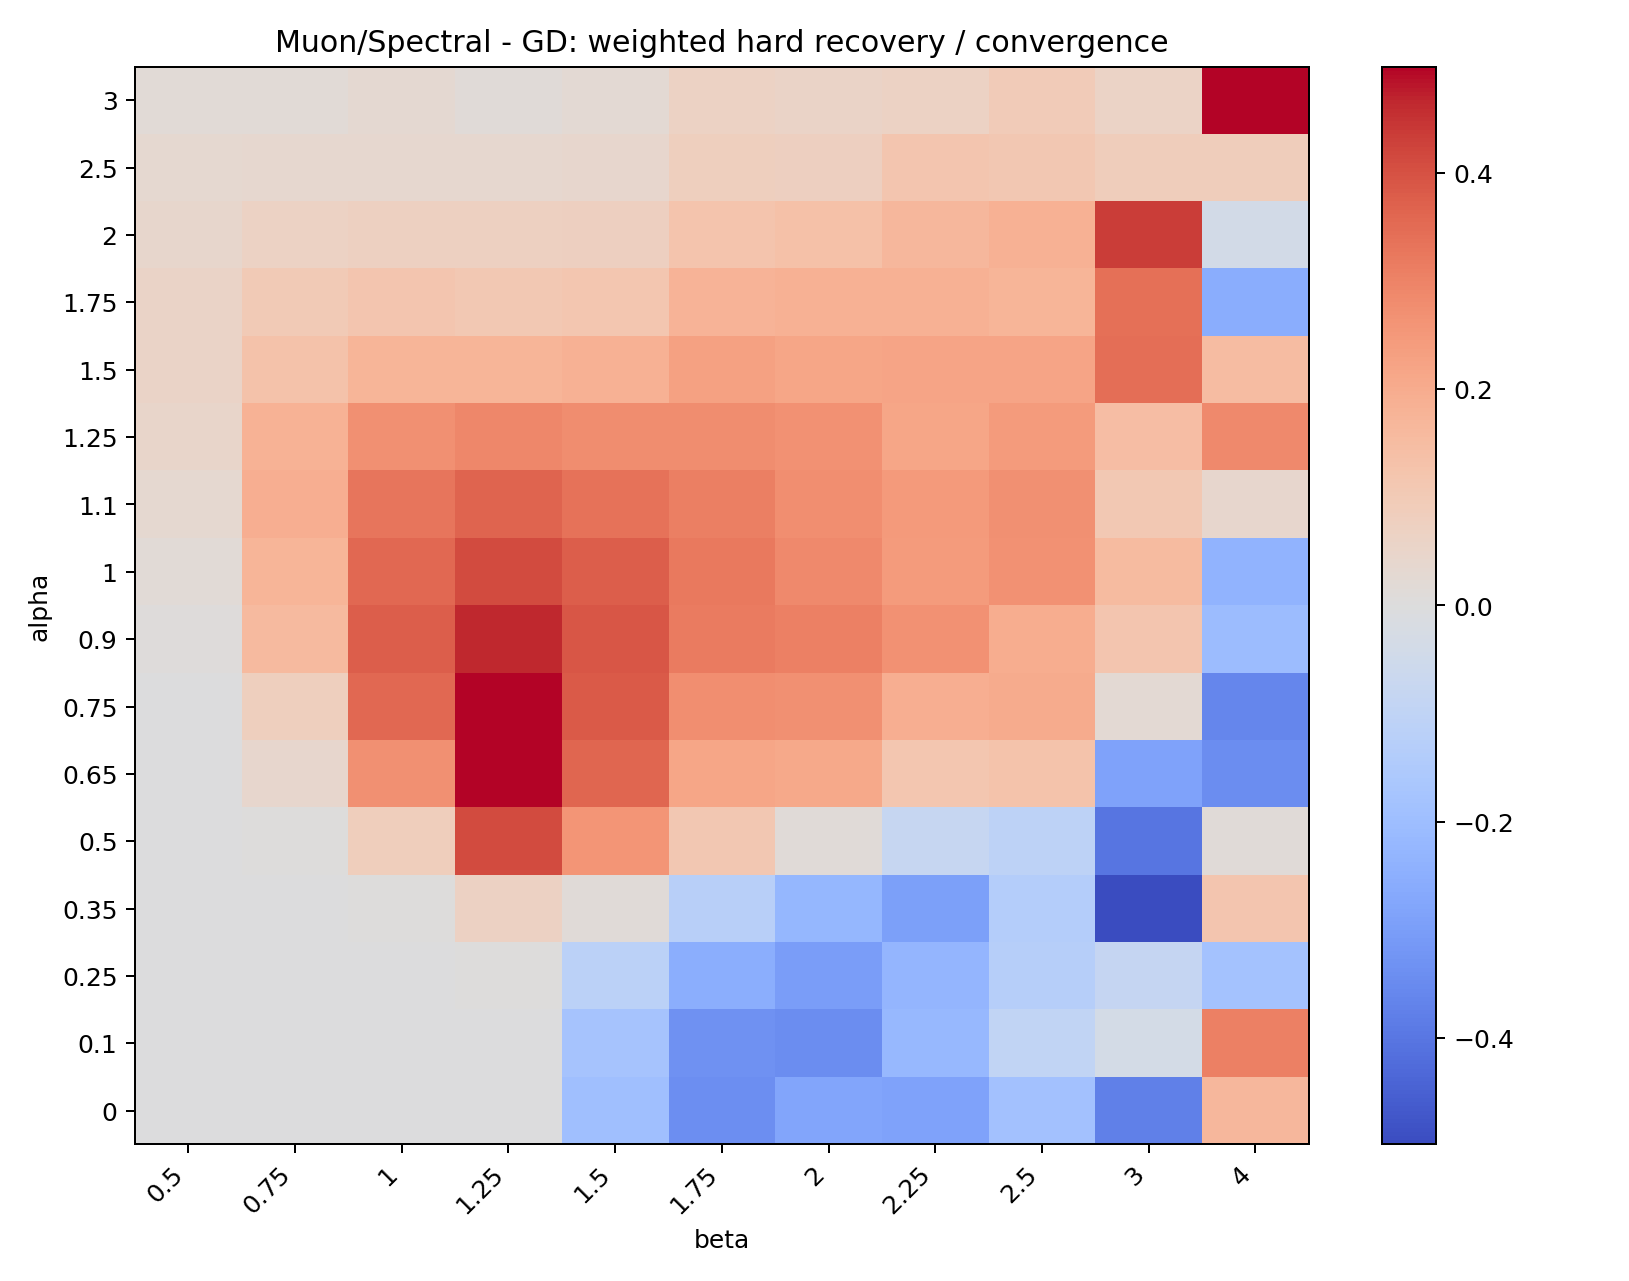
\includegraphics[width=\linewidth]{figures/fraction_heatmaps/unit_weighted_recovered_mass_fraction_spectral_minus_gd.png}
  \caption{Muon $-$ GD}
\end{subfigure}
\caption{Experiment II fraction of convergence-reference weighted hard
recovery.  Muon/Spectral often captures nearly all of the recoverable
weighted mass in one step, especially when the distribution is sufficiently
head-concentrated.}
\label{fig:exp2-frac-weighted}
\end{figure}

\begin{figure}[H]
\centering
\begin{subfigure}[t]{0.32\textwidth}
  \centering
  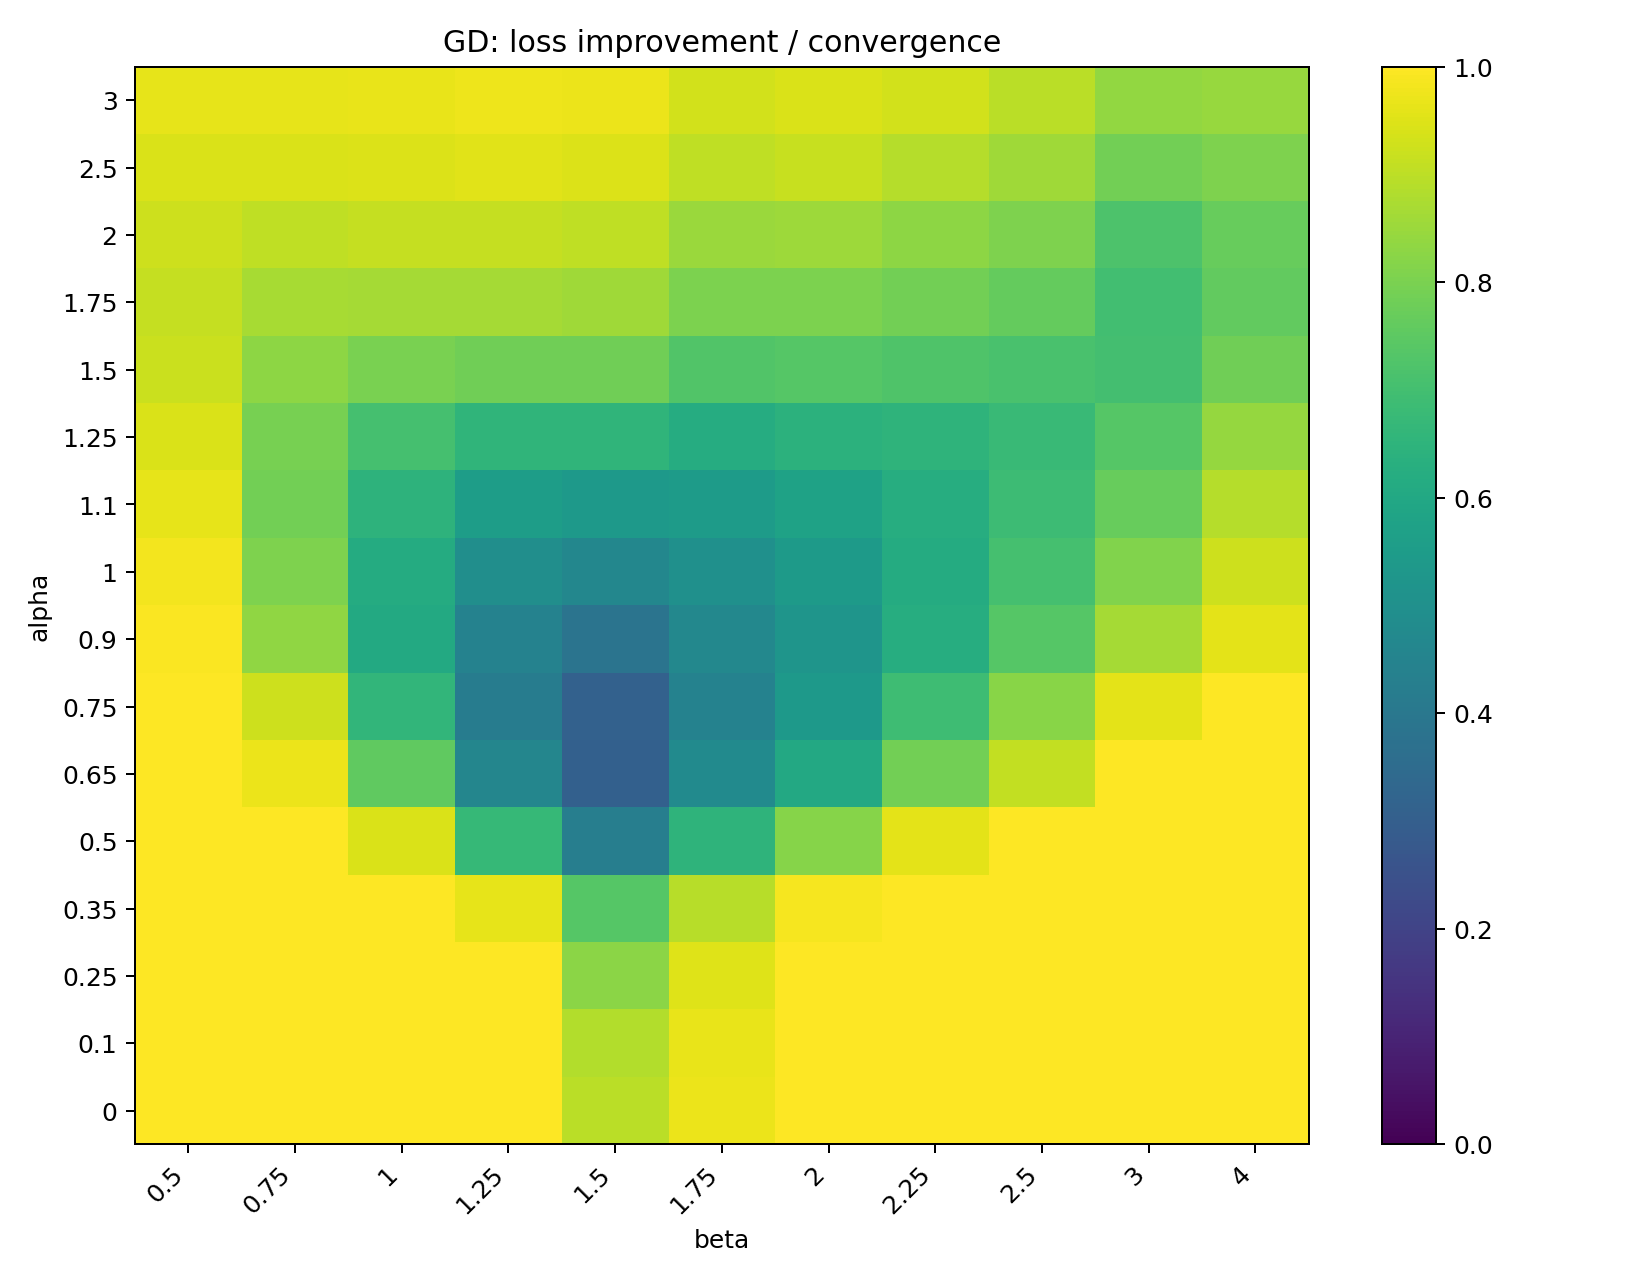
\includegraphics[width=\linewidth]{figures/fraction_heatmaps/loss_improvement_fraction_gd.png}
  \caption{GD}
\end{subfigure}
\hfill
\begin{subfigure}[t]{0.32\textwidth}
  \centering
  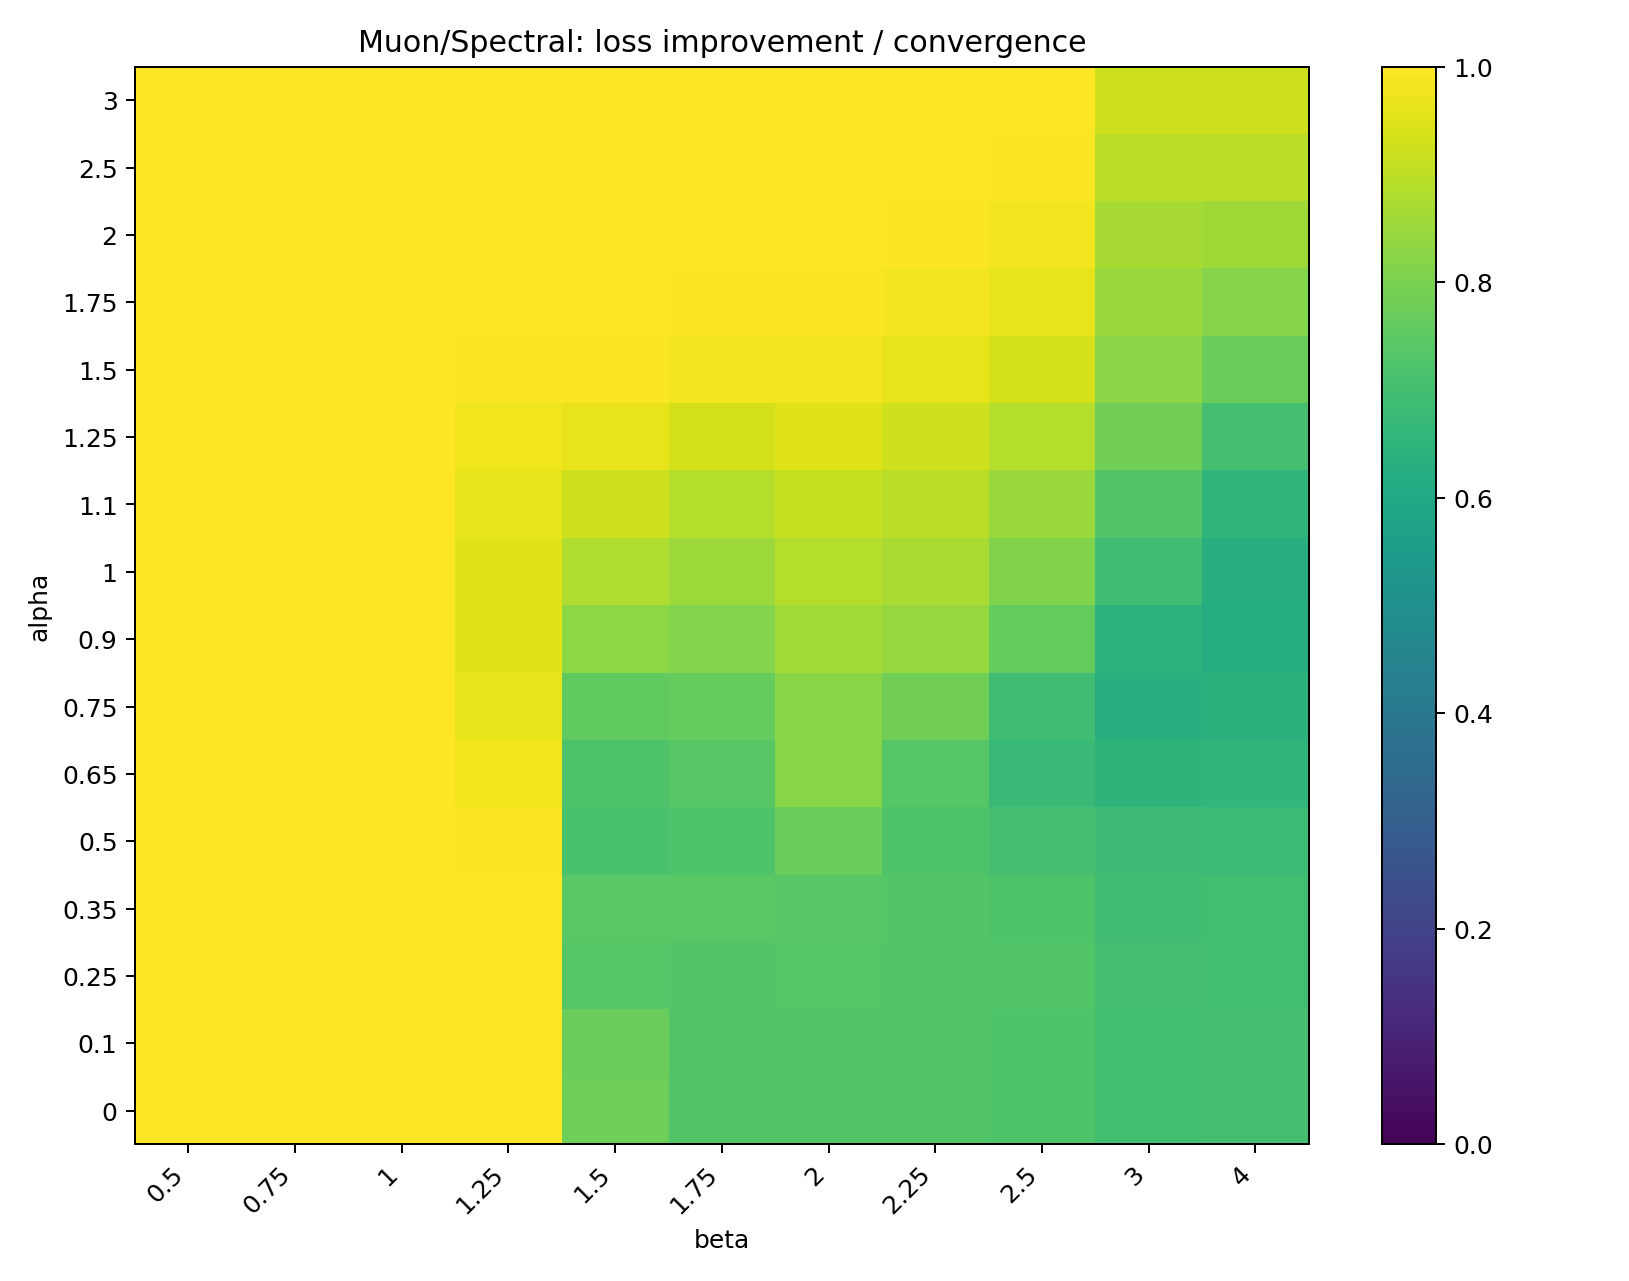
\includegraphics[width=\linewidth]{figures/fraction_heatmaps/loss_improvement_fraction_spectral.png}
  \caption{Muon/Spectral}
\end{subfigure}
\hfill
\begin{subfigure}[t]{0.32\textwidth}
  \centering
  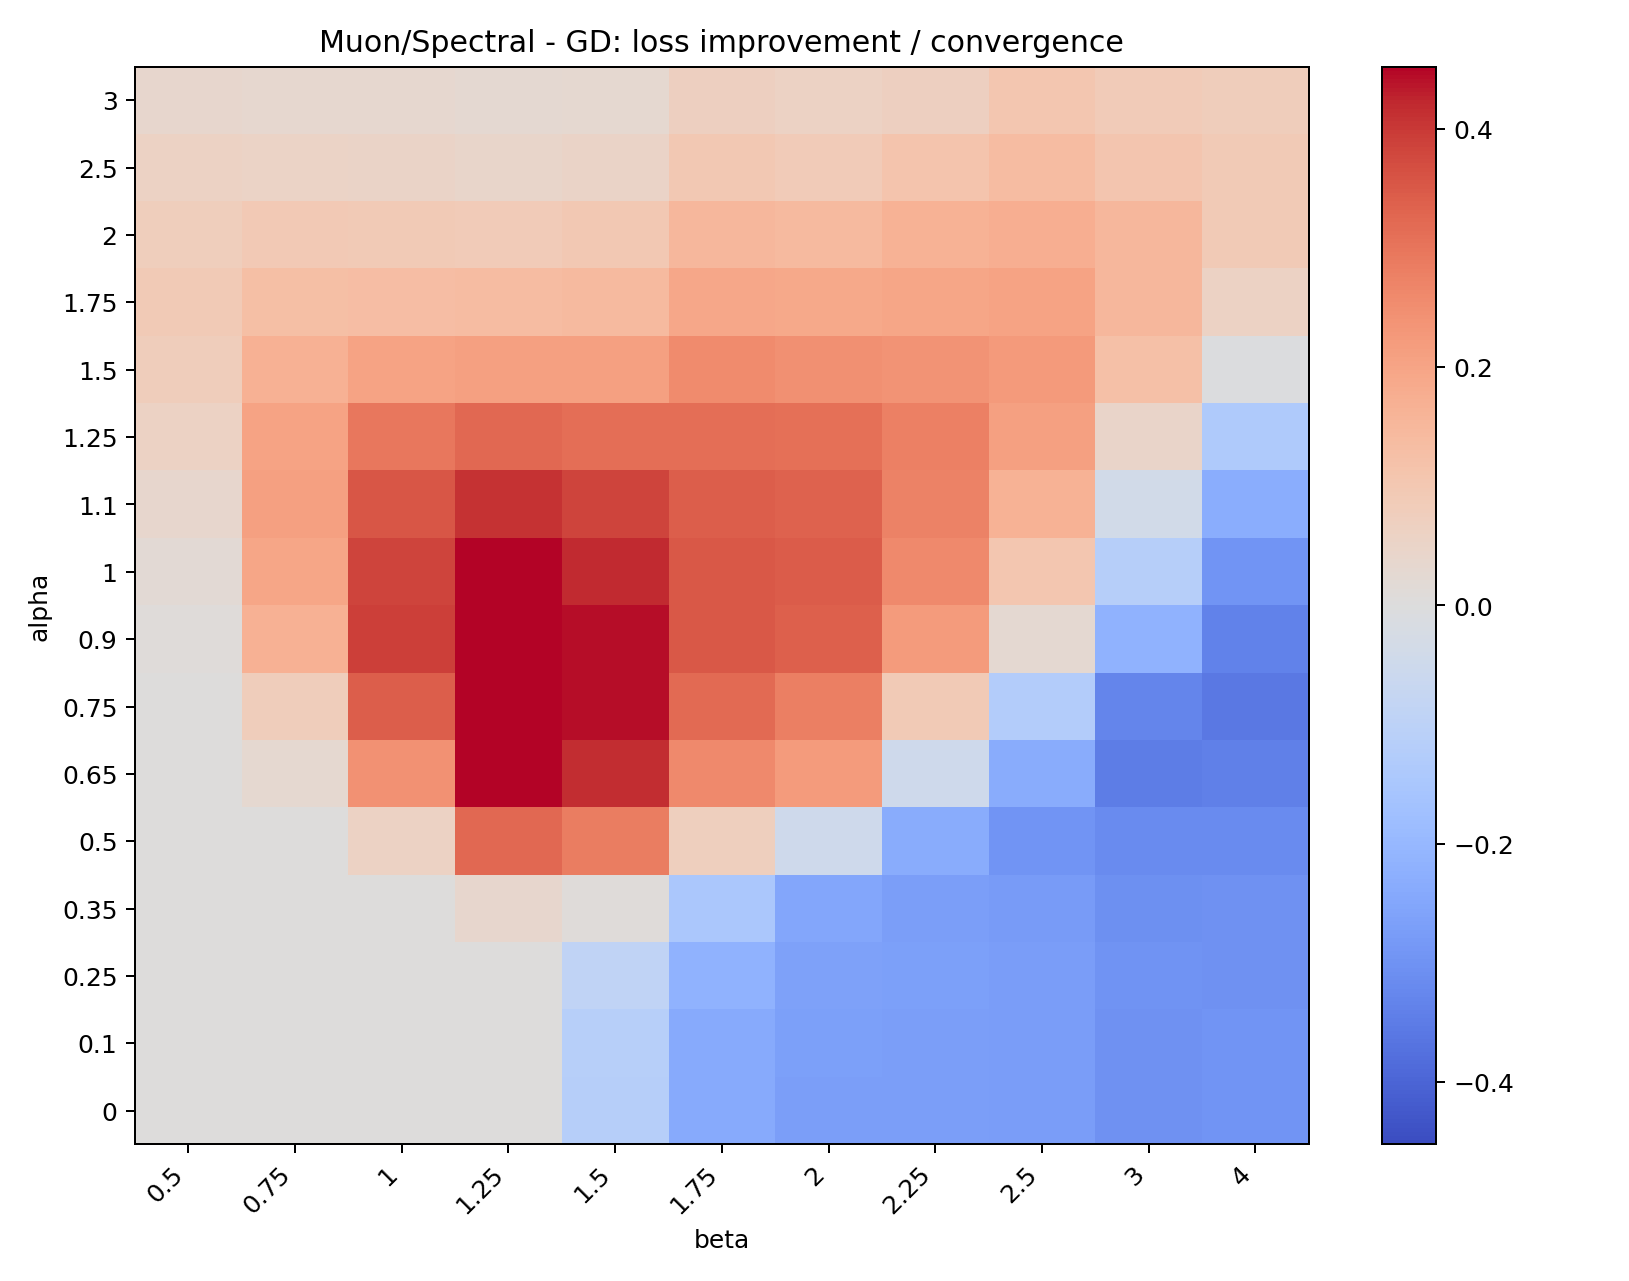
\includegraphics[width=\linewidth]{figures/fraction_heatmaps/loss_improvement_fraction_spectral_minus_gd.png}
  \caption{Muon $-$ GD}
\end{subfigure}
\caption{Experiment II fraction of convergence-reference loss improvement.
The yellow regions in the Muon/Spectral panel show regimes where one step
already achieves essentially the same loss decrease as the optimized
reference.}
\label{fig:exp2-frac-loss}
\end{figure}

\begin{figure}[H]
\centering
\begin{subfigure}[t]{0.32\textwidth}
  \centering
  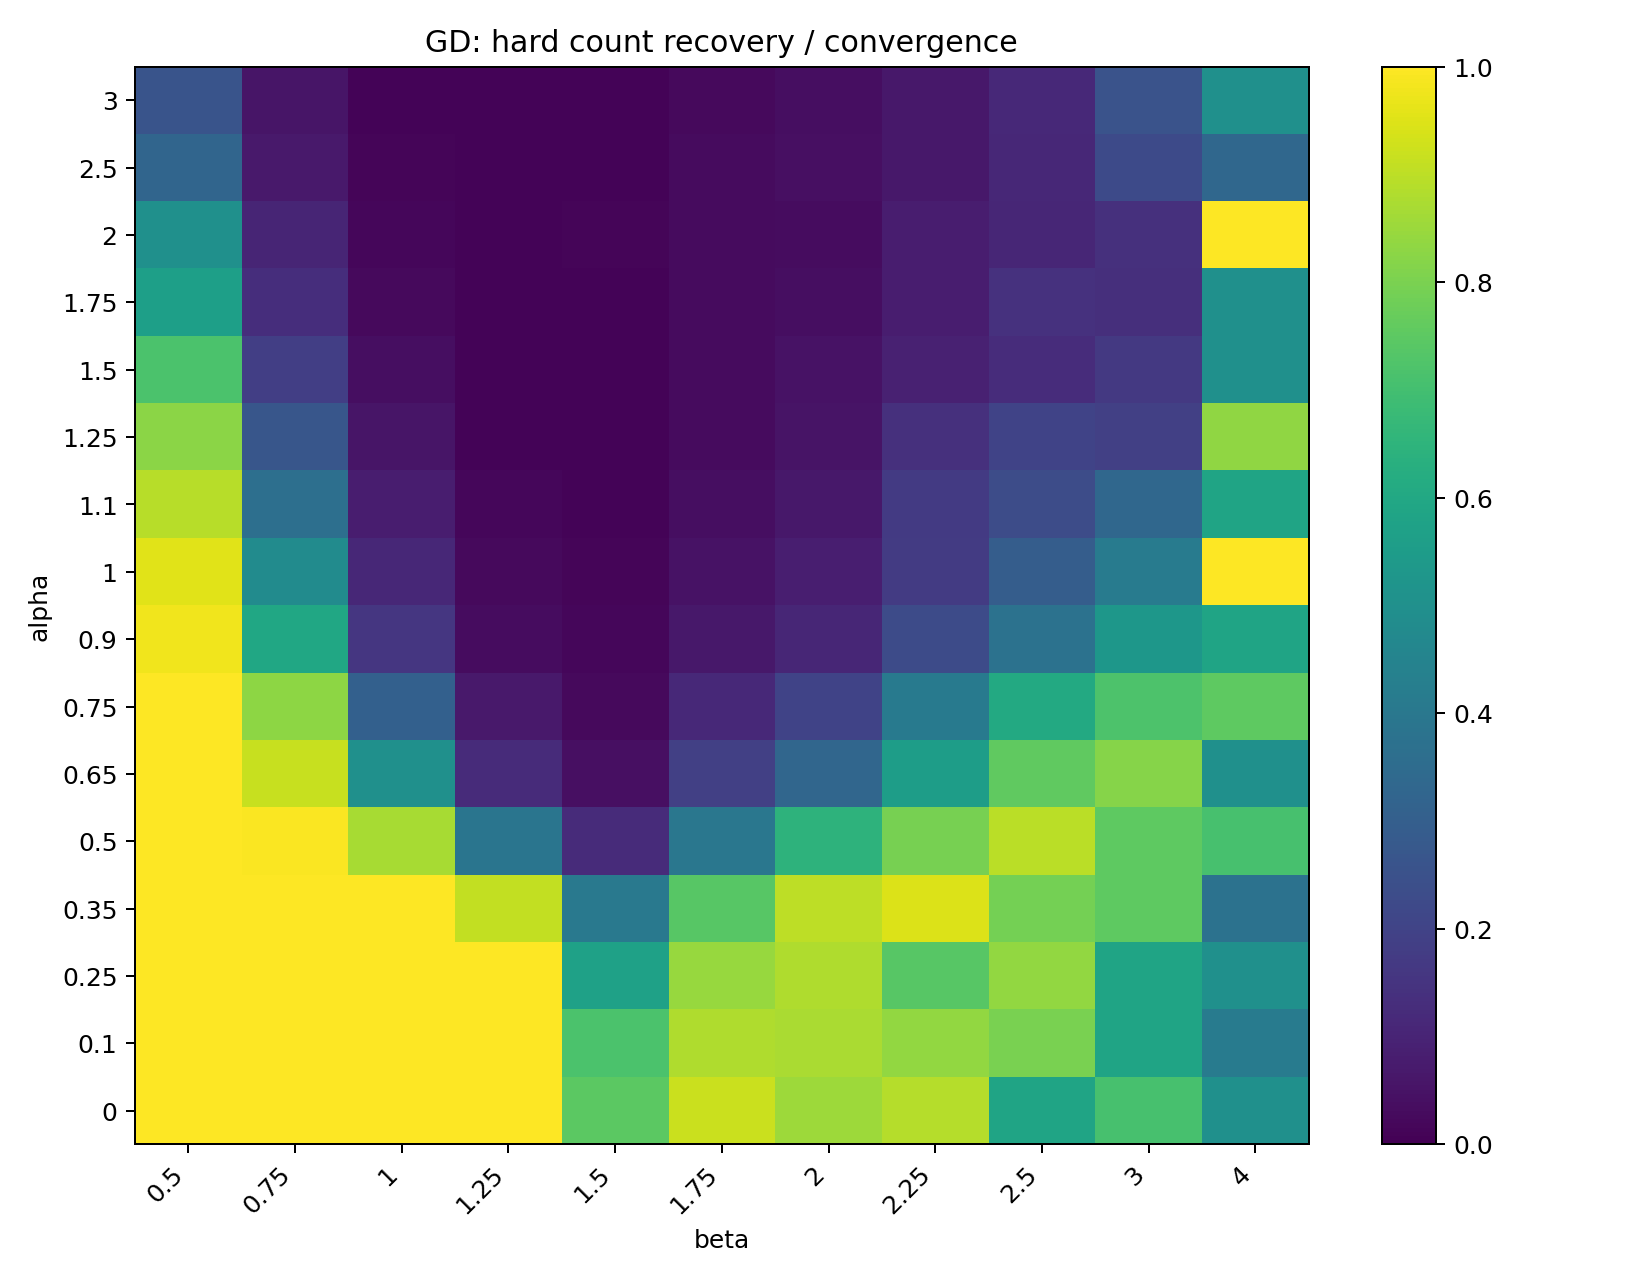
\includegraphics[width=\linewidth]{figures/fraction_heatmaps/unit_recovered_fraction_fraction_gd.png}
  \caption{GD}
\end{subfigure}
\hfill
\begin{subfigure}[t]{0.32\textwidth}
  \centering
  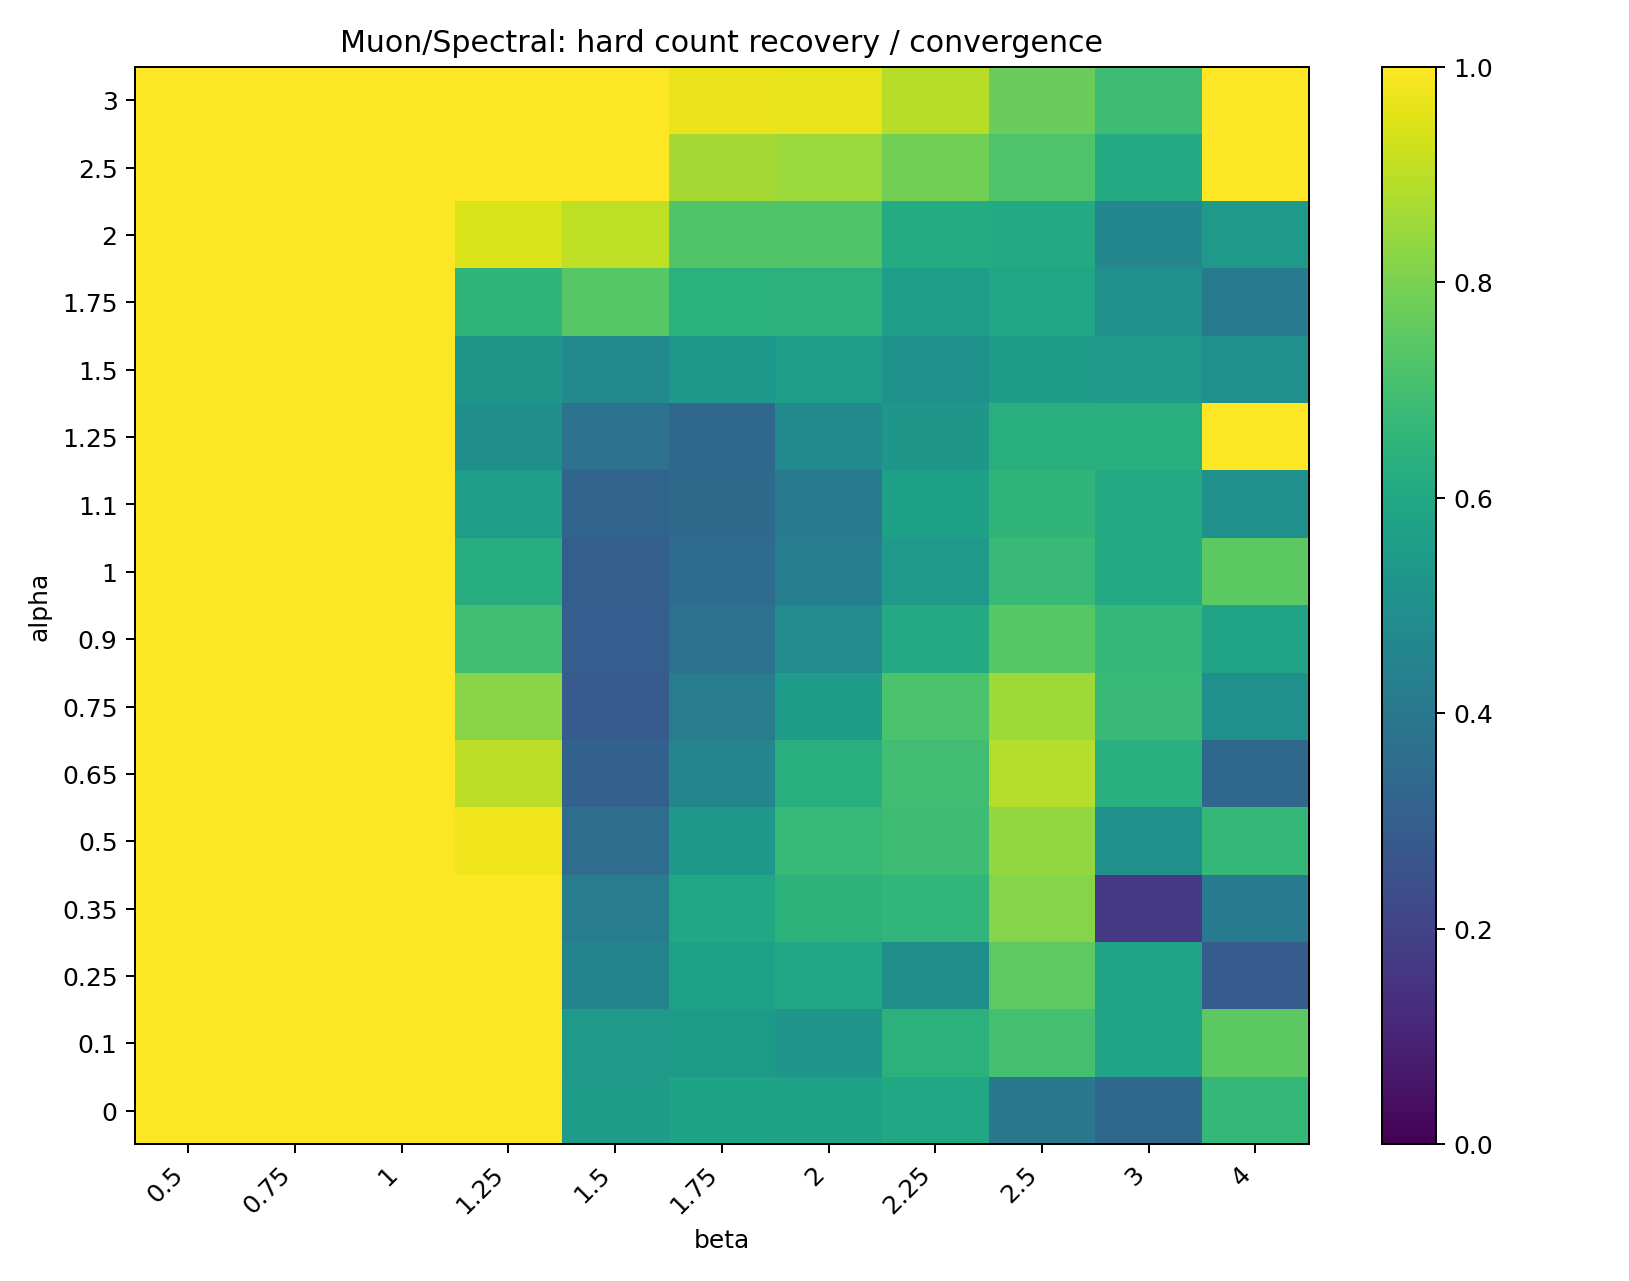
\includegraphics[width=\linewidth]{figures/fraction_heatmaps/unit_recovered_fraction_fraction_spectral.png}
  \caption{Muon/Spectral}
\end{subfigure}
\hfill
\begin{subfigure}[t]{0.32\textwidth}
  \centering
  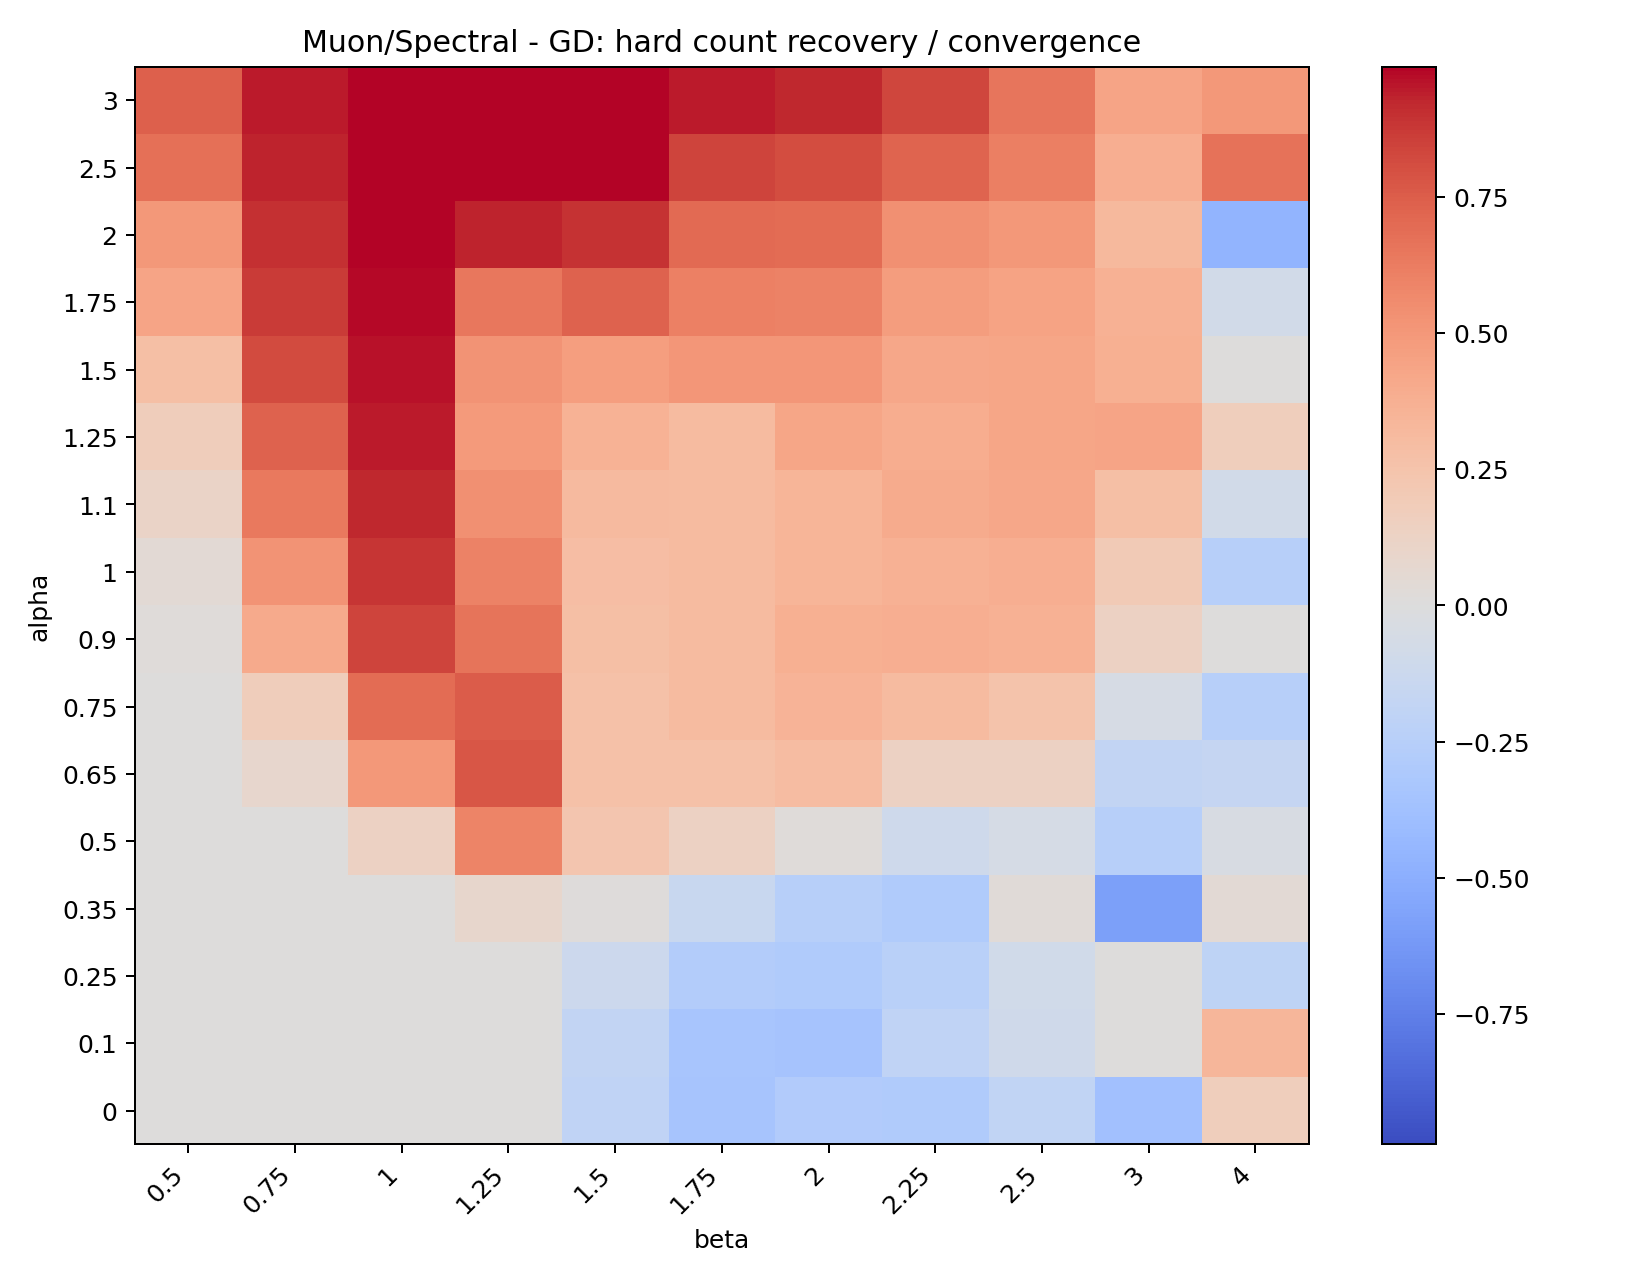
\includegraphics[width=\linewidth]{figures/fraction_heatmaps/unit_recovered_fraction_fraction_spectral_minus_gd.png}
  \caption{Muon $-$ GD}
\end{subfigure}
\caption{Experiment II fraction of convergence-reference hard count recovery.
This remains the strictest metric, but Muon/Spectral still captures a much
larger fraction of the reference count recovery than GD in many transition
regimes.}
\label{fig:exp2-frac-count}
\end{figure}

\subsection{Numerical summary}

Table~\ref{tab:exp2-method-summary} reports aggregate seed-median fractions
over all 176 grid cells.  Table~\ref{tab:exp2-threshold-main} reports how
many grid cells achieve at least 90\% or 95\% of the convergence reference.

\begin{table}[H]
\centering
\caption{Experiment II aggregate one-step fractions of the convergence
reference.  Values are medians over the seed-median grid cells.}
\small
\begin{tabular}{lrrrr}
\toprule
Method & $F_{\rm loss}$ & $F_{\rm WHR}$ & $F_{\rm HCR}$ & $F_{\rm WSR}$ \\
\midrule
GD & 0.886 & 0.814 & 0.350 & 0.959 \\
Muon/Spectral & 0.956 & 0.953 & 0.690 & 1.001 \\
\bottomrule
\end{tabular}
\label{tab:exp2-method-summary}
\end{table}

\begin{table}[H]
\centering
\caption{Experiment II count of largest-$d$ grid cells whose seed-median
one-step fraction exceeds the specified threshold.  There are 176 grid cells
per method.}
\small
\begin{tabular}{llrrrr}
\toprule
Metric & Threshold & GD cells & GD frac. & Muon cells & Muon frac. \\
\midrule
$F_{\rm loss}$ & 0.90 & 83 & 0.472 & 97 & 0.551 \\
$F_{\rm loss}$ & 0.95 & 62 & 0.352 & 90 & 0.511 \\
$F_{\rm WHR}$ & 0.90 & 62 & 0.352 & 102 & 0.580 \\
$F_{\rm WHR}$ & 0.95 & 42 & 0.239 & 89 & 0.506 \\
$F_{\rm HCR}$ & 0.90 & 28 & 0.159 & 65 & 0.369 \\
$F_{\rm HCR}$ & 0.95 & 23 & 0.131 & 62 & 0.352 \\
\bottomrule
\end{tabular}
\label{tab:exp2-threshold-main}
\end{table}

\section{Conclusion}

The combined evidence supports a one-step-centered empirical picture.  In
low and moderate $\beta$ regimes, one step already recovers most or all of
the memory.  In transition regimes, Muon/Spectral substantially expands the
one-step-good region relative to GD.  When one-step performance is compared
against a separately optimized mini-batch convergence reference, a single
Muon/Spectral update often captures almost all of the reference loss
improvement and weighted recovery.  Large-$\beta$ exact runs remain limited
by the maximum feasible dimension, so weak low-alpha recovery there should
not be used as evidence for a meaningful multi-step convergence boundary.


\end{document}
